% input files


% document's head
\vspace{2cm}

\begin{center}
    \LARGE \textsc{Конспект второго тома курса теоретической физики <<Теория поля>>}
\end{center}

\hrule

\begin{flushright}
    \begin{tabular}{rr}
    % written by:
        \textbf{Авторы}: 
        & Хоружий Кирилл \\
        & Примак Евгений \\
        &\\
    % date:
        \textbf{От}: &
        \textit{\today}\\
    \end{tabular}
\end{flushright}

\thispagestyle{empty}
\tableofcontents
\newpage



%%%%%%%%%%%%%%%%%%%%%%%%%%%%%%%%%%%%%%%%%%%%%%%%%%%%%%%%%%%%%%%%%%%%%%%%%%%%%%%%%%%
\secnum{1}{Криволинейные координаты и кинематика} % 1-6
%%%%%%%%%%%%%%%%%%%%%%%%%%%%%%%%%%%%%%%%%%%%%%%%%%%%%%%%%%%%%%%%%%%%%%%%%%%%%%%%%%%

\sbsnum{1}{Кинематика точки}
Для точки $P$ движущейся относительно некоторого неподвижного тела (свяжем с ним точку $O$), можно ввести следующие характеристики:
\begin{to_def}[Радиус вектор, скорость и ускорение точки $P$]
	\begin{equation*}
	\vc{r} = \overrightarrow{O P},
	\hspace*{1 cm}
	\vc{v} = \frac{d \vc{r}}{d \vc{t}},
	\hspace*{1 cm}
	\vc{w} =  \frac{d \vc{v}}{d t} = \frac{d^2 \vc{r}}{d t^2}.
\end{equation*}	
\end{to_def}

\begin{to_def}
	Для задания движения точки, зная её траекторию, можно сопоставить ей дуговую координату $\sigma (t)$ и получить выражения для скорости и ускорения, выраженные в осях \textit{естественного трёхгранника} $\vc{\tau}, \vc{n}, \vc{b}$.
	Таким образом для $\vc{r} = \vc{r}(\sigma(t))$:
	\begin{equation*}
		\vc{\tau} (\sigma) = \frac{d \vc{r}}{d \sigma}, 
		\hspace*{1 cm} 
		\frac{d \vc{\tau}}{d \sigma} = \frac{1}{\rho} \vc{n} (\sigma),
	\end{equation*}
	где $\rho$ -- радиус кривизны. Для кривой в $\mathbb{R}^3$ добавим ещё вектор $b$ для правой тройки. Таким образом получим формулы Френе:
	\begin{equation*}
		\frac{d \vc{\tau}}{d s} = \frac{1}{\rho} \vc{n},
		\hspace*{1 cm}
		\frac{d \vc{n}}{d s} = - \frac{1}{\rho} \vc{\tau} + \varkappa \vc{b},
		\hspace*{1 cm}
		\frac{d \vc{b}}{d s} = - \varkappa \vc{n}.
	\end{equation*}
\end{to_def}

Таким образом сможем в компонентах трёхгранника выписать скорость и ускорение точки:
\begin{gather*}
   \vc{v} = \frac{d \vc{r}}{d t} = \frac{d \vc{r}}{d \sigma} \frac{d \sigma}{d t} = v_\tau \vc{\tau}
   \\
   \vc{w} = \frac{d \vc{v}}{d t} = \frac{d_\tau}{d t} \vc{\tau} + v_\tau \frac{d \vc{\tau}}{d \sigma} \frac{d \sigma}{d t} = \frac{d^2 \sigma}{d t^2} \vc{\tau} + \frac{v_\tau^2}{\rho} \vc{n}.
\end{gather*}
Как видно, ускорение точки представилось в видео $w = w_n + w_\tau $ --- \textit{нормальной} и \textit{тангенциальной} составляющей.

\begin{to_lem}[Из матана]
	Для $f_i \in  C^2 \colon U \mapsto V$, если $X$ -- касательный вектор в точке $p \in U$, то $X(f)$ можно определить как:
	\begin{equation*}
		X(f) = X(x^i) \frac{\partial f(p)}{\partial x^i}, \text{ а координаты этого вектора в криволинейных координатах: } X = X^i \frac{\partial}{\partial x^i}.
	\end{equation*}
\end{to_lem}

Каждую материальную точку можем определить $\vc{r}_1, \ldots, \vc{r}_N$ -- итого $\mathbb{R}^{3N}$. Но есть некоторые ограничения вида
\begin{equation*}
    f_i (\vc{r}, t) = 0.
\end{equation*}
Вложим в фазовое пространство многообразие $M$, в котором локально всё хорошо. Тогда
$\dim M = n$ -- число степеней свободы, а параметризация $q_1, \ldots, q_N$ -- криволинейные координаты. В каждой $A \in M$ верно, что $\dot{\vc{q}} \in TM_A$, то есть
\begin{equation*}
    TM = \bigcup_q T_qM \ni (q, \dot{q})
\end{equation*}

И так, движение точки можно задать, если её криволинейные координаты --- известне функции $q(t)$.
\begin{equation*}
	\vc{r} = \vc{r}(q_1, q_2, q_3) = x \vc{i} + y \vc{j} + z \vc{k}.
\end{equation*}

\begin{to_def}
	\textit{Коэффициентами Ламе} такие $H^i$. C их помощью удобно выразить единичные базисные векторы криволинейных координат: 
	\begin{equation*}
		H_i = \left|\frac{\partial \vc{r}}{\partial q^i} \right| = \sqrt{\left(\frac{\partial x}{\partial q^i}\right)^2 + \left(\frac{\partial y}{\partial q^i}\right)^2 + \left(\frac{\partial z}{\partial q^i}\right)^2}.
		\hspace*{1 cm}
		e^i = \frac{1}{H_i} \frac{\partial \vc{r}}{\partial q^i}.
	\end{equation*}
\end{to_def}

Далее будем координатными векторами называть $\vc{g}_i(\vc{r}) = \frac{\partial \vc{r}}{\partial q^i}$. Разложение произвольного вектора по локальному базису имеет вид:
\begin{equation*}
	\vc{a} = a^i \vc{g}_i = a_j \vc{g}^j.
\end{equation*}
Здесь $\vc{g}^j$ --- векторы двойственного базиса к базису из $\vc{g}_i$. В двойственном же (взаимном) базисе из матана мы видели:
\begin{equation*}
	X(f) = d f (X) = \partial_x f,
	\hspace*{1 cm}
	d x^i (\frac{\partial}{\partial x^j}) = \frac{\partial x^i}{\partial x^j} = \delta_j^i,
	\hspace*{1 cm}
	a = a_i d x^i.
\end{equation*}
Таким образом получаем скорость точки и её ковариантную компоненту:
\begin{equation*}
	\vc{v} = \frac{d \vc{r}}{d t} = \frac{\partial \vc{r}}{\partial q^i} \frac{d q^i}{d t} = \vc{g}_i \dot{q}^i,
	\hspace*{1 cm}
	v^i = \vc{q}^i.
\end{equation*}
И для ускорения:
\begin{equation*}
	w_k = \left(\frac{d \vc{v}}{d t}\right)_k = \frac{(d \vc{v})_k}{d t} = g_{k j} \frac{d v^j}{d t} + \Gamma_{k i j} v^j v^i.
\end{equation*}


\sbsnum{2}{Описание движения твёрдого тела}
\begin{to_def}
	\textit{Твёрдое телое} --- множество точек, расстояние между которыми не меняется: $\forall j, j, t \colon \vc{|r}_i(t) - \vc{r}_j| = \const$. 
\end{to_def}

Точка $O$ это полюс. Во-первых перенесем начало координат в $O$. Введём систему координат $O_{\xi\nu\zeta}$ связанную с телом, -- тело относительно неё не движется
\begin{equation*}
	 \vc{r} = \vv{OA}, \, \vc{\rho} = \vv{OA} = \const \text{ в $O_{\xi\nu\zeta}$},
    \hspace{0.5cm} \Rightarrow \hspace{0.5cm} 
    \vc{r}(t) = R(t) \vc{\rho}.
\end{equation*}

\begin{wrapfigure}{r}{0.25\textwidth}
  \begin{center}
        \vspace{-10 mm}
        \includegraphics[width=0.9\linewidth]{img/eu_angles.png}
  \end{center}
    \caption{Углы Эйлера}
\end{wrapfigure}

Ортогональность матрицы $R$ даёт возможность описать её тремя независимыми параметрами. Один из вариантов сделать это -- углы Эйлера. 

Пусть начальная ПДСК $(x, y, z)$, а конечная -- $(X, Y, Z)$, при чём $xy \cap XY = ON$ -- линия узлов.
\begin{align*}
    1) \hspace{0.25cm}  \alpha &\colon Ox \to ON, &\text{ угол \textit{прецессии}}; \\
    2) \hspace{0.25cm}  \beta  &\colon Oz \to OZ, &\text{ угол \textit{нутации}}; \\
    3) \hspace{0.25cm}  \gamma &\colon OX \to ON, &\text{ угол \textit{собственного вращения}}.
\end{align*}
Повороты системы на эти углы называются прецессия, нутация и поворот на собственный угол (вращение). 

\phantom{42}

\noindent
Матричная запись углов Эйлера:
\begin{equation*}
    R_Z(\alpha) = \begin{pmatrix}
        \cos \alpha & - \sin \alpha & 0 \\
        \sin    a & \cos\alpha & 0 \\
        0 & 0 & 1\\
    \end{pmatrix},
\end{equation*}
\begin{equation*}
    R_X(\beta) = \begin{pmatrix}
        1 & 0 & 0 \\
        0 & \cos \beta & -\sin \beta \\
        0 & \sin \beta & \cos \beta \\
    \end{pmatrix},
    \hspace{1cm} 
    R_Z (\gamma) = \begin{pmatrix}
        \cos(\gamma) & - \sin \psi & 0 \\
        \sin \gamma & \cos \gamma & 0\\
        0 & 0 & 1
    \end{pmatrix}.
\end{equation*}

\begin{to_thr}[Теорема Эйлера]
     Произвольное перемещение твердого тела, имеющего неподвижную точку, можно осуществить посредством вращения вокруг некоторой оси, проходящей через эту точку. 
\end{to_thr}

\begin{to_thr}[Теорема Шаля]
     Самое общее перемещение твердого тела разлагается на поступательное перемещение, при котором произвольно выбранный полюс переходит из своего первоначального положения в конечное, и на вращение вокруг некоторой оси, проходящей через этот полюс. Это разложение можно совершить не единственным способом, выбирая за полюс различные точки тела; при этом направление и длина поступательного перемещения будут изменяться при выборе различных 
полюсов, а направление оси вращения и угол поворота вокруг нее не зависят от выбора полюса. 
\end{to_thr}

\begin{to_thr}[Теорема Моцци]
\label{thr_moz}
     Самое общее перемещение твердого тела является винтовым перемещением.
\end{to_thr}

\begin{to_con}[Теорема Бернулли-Шаля]
     Самое общее перемещение плоской фигуры в своей плоскости есть либо поступательное перемещение, либо вращение вокруг точки. Эта точка называется центром конечного вращения.
\end{to_con}

\sbsnum{3}{Приложения к твердому телу}
Проведём два вектора $\vc{r}_A, \vc{r}_O$:
\begin{equation*}
    \vc{r}_A = \vc{r}_O + \vc{r} = \vc{r}_O + R(t) \vc{\rho}
    \hspace{0.5cm} \overset{d / dt}{\Rightarrow} \hspace{0.5cm} 
    \vc{v}_A = \vc{v}_O + \dot{R} \rho = \vc{v}_O + \dot{R} R^{-1}\vc{r}
\end{equation*}
но,
\begin{equation*}
    RR\T = E, \dot{R} R\T + R \dot{R}\T = 0, \dot{R} R\T = - R \dot{R}\T,
    (\dot{R} R^{-1})\T = - \dot{R} R^{-1}.
\end{equation*}

То есть $\dot{R} R^{-1}$ кососимметрична. Тогда пусть
\begin{equation*}
    \dot{R} R^{-1} = \Omega = \begin{pmatrix}
        0 & -\omega_z & w_y \\
        w_z & 0 & -\omega_x \\
        -\omega_y & \omega_x & 0\\
    \end{pmatrix}
\end{equation*}
Таким образом мы доказали следующую теорему.

\begin{to_thr}[формула Эйлера]
\label{eq_euler}
    Существует единственный вектор\footnote{
        Псевдоветор же, нет?
    } $\vc{\omega}$, называемый \textbf{угловой скоростью тела}, с помощью которого скорость $\vc{v}$ точки тела может быть представлена в виде
    \begin{equation*}
        \vc{v}_A = \vc{v}_O + \vc{\omega} \times \vc{r}
        \hspace{0.5cm} \text{--} \hspace{0.5cm} \text{\textbf{формула Эйлера}.}
    \end{equation*}
\end{to_thr}

Тогда, например, при постоянном радиус векторе верно, что
\begin{equation*}
    \vc{v}_A = \frac{d \vc{a}}{dt} = \vc{\omega} \times \vc{a},
    \hspace{0.5cm} \text{при условии $a = \const$}.
\end{equation*}

Можно вывести ускорение точки твёрдого тела
\begin{align*}
    \vc{\mathrm{w}}_A &= \vc{\mathrm{w}}_O + \frac{d \vc{\omega}}{dt} \times \vc{r} + \vc{\omega} \times \frac{d \vc{r}}{dt}, \\
    \vc{\mathrm{w}}_A &= \vc{\mathrm{w}}_O + \vc{\varepsilon} \times \vc{r} + \vc{\omega} \times \left(\vc{\omega} \times \vc{r} \right)
    \hspace{0.5cm} \text{--} \hspace{0.5cm} \text{\textbf{формула Ривальса},}
\end{align*}
где $\vc{\varepsilon} = d \vc{\omega} / d t$ -- \textit{угловое ускорение}.

\subsubsection*{Вращение вокруг неподвижной оси}
\begin{wrapfigure}{r}{0.25\textwidth}
  \begin{center}
        \vspace{-10 mm}
        \includegraphics[width=0.9\linewidth]{img/stable_axis.png}
  \end{center}
    \caption{Ориентация тела относительно неподвижной системы координат}
\end{wrapfigure}
Пусть точка $P$ задана в связанной системе координат радиус-вектором $\rho$:
\begin{equation*}
    \vc{r} = A \vc{\rho},
    \hspace*{0.5 cm}
    A = \begin{pmatrix}
            \cos \varphi & - \sin \varphi & 0 \\
            \sin \varphi & \cos \varphi & 0 \\
            0 & 0 & 1
        \end{pmatrix}.
\end{equation*}
После прямых вычислений получаем, что
\begin{equation*}
    \dot{A} A^{-1} = 
    \begin{pmatrix}
        0 & - \dot{\varphi} & 0 \\
        \dot{\varphi} & 0 & 0 \\
        0 & 0 & 0    
    \end{pmatrix},
    \hspace*{1 cm}
    \dot{\omega} = \begin{pmatrix}
        0 \\ 0 \\ \dot{\varphi}
    \end{pmatrix},
    \hspace*{1 cm}
    \vc{\varepsilon} = \begin{pmatrix}
        0 \\ 0 \\ \ddot{\varphi}    
    \end{pmatrix}.
\end{equation*}
Таким образом получили, что угловая скорость $\vc{\omega}$ направлена по оси вращения по правилу буравчика. Угловое ускорение $\vc{\varepsilon}$ коллинеарно $\vc{\omega}$.

Для вычисления $w_P$ примем $O$ за полюс. Тогда $v_O= 0$, что значит $\vc{v} = \vc{\omega} \times \vc{r}$ -- вектор скорости перпендикулярен оси вращения. И из формулы Ривальса:
\begin{equation*}
    w = \underbrace{\vc{\varepsilon} \times \vc{r}}_{w_\text{вр}} + \underbrace{\vc{\omega} \times \vc{v}}_{w_\text{ос}},
    \hspace*{1 cm}
\end{equation*}
где \textit{вращательное} ускорение $w_\text{вр} = \ddot{|\varphi}| d$, а \textit{осестремительное} $w_\text{ос} = \omega^{2}d$, а $d$ --- радиус окружности, по которой движется $P$.

\subsubsection*{Движение вокруг неподвижной точки}
Точка $O$ --- неподвижна, тогда $v_0 = 0, \ w_0 = 0 $ и формулы, полученные в разделе выше одни и те же. Однако стоит ввести пару определений:
\begin{to_def}
    \textit{Мгновенная ось вращения} --- ось на которой в данный момент времени лежит $\vc{\omega}$, которая в свою очередь --- \textit{мгновенная угловая скорость}. 
\end{to_def}
\begin{to_def}
    При своём движении мгновенная ось вращения описывает в теле коническую поверхность --- \textit{подвижный аксоид}, а в абсолютном пространстве --- \textit{неподвижный аксоид}.
    При движении тела подвижный аксоид катится по неподвижному без скольжения.
\end{to_def}

Годограф $\vc{\omega}$ лежит на неподвижном аксоиде. 
Так как $\vc{\varepsilon} = \vc{\dot{\omega}}$, то $\vc{\varepsilon}$ направлено по касательной к годографу и вовсе не обязательно по мгновенной оси вращения. 
Если $\vc{\omega} = \omega \vc{e}$, для единичного $\vc{e}$, то $\vc{\varepsilon} = \dot{\omega} \vc{e} +\omega \vc{\dot{e}}$.
Если мгновенная ось вращается вокруг $O$ с $\vc{\Omega}$, то $\omega \vc{\dot{e}} = \vc{\Omega} \times \vc{\omega}$.

Вновь воспользовавшись формулой Ривальса вычислим осетремительное ускорение, для $Q$ --- точке на мгновенной оси вращения:
\begin{equation*}
    w_\text{ос} = \vc{\omega}\times (\vc{\omega} \times \vc{r}) = \omega^2 \vc{e} \times (\vc{e} \times \vc{r}) = \omega^2[\vc{e} (\vc{e} \cdot \vc{r}) - \vc{r}] = \omega^2 (\overrightarrow{O Q} - \vc{r}) = \omega^2 \vc{l}.
\end{equation*}
Таким образом получили, что $w_\text{ос}$ совпадает при вращении, как если бы ось было неподвижной.

\subsubsection*{Плоское движение}
\begin{to_def}
    \textit{Плоское движение} --- движение тела, при котором все его точки перемещаются в плоскостях параллельных некоторой неподвижной плоскости.
\end{to_def}

Плоская фигура вынужденно двигаясь в своей плоскости имеет три степени свободы: $(x,y,\varphi)$. Скорости и ускорения всё так же ищутся по общем формулам, но в данном случае полезно рассмотреть несколько теорем:
\begin{to_thr}
    При плоском движении фигуры во мгновение $t$, если движение не поступательно, то $\exists ! C$-точка, такая что $v_C =0$, а остальные точки тела движутся как при вращении вокруг $C$.
\end{to_thr}
\begin{to_def}
    Такая точка $C$ --- называется \textit{мгновенным центром скоростей}.
\end{to_def}

\begin{to_thr}
    Для движения плоской фигуры в своей плоскости. Если в момент $t$ $\dot{\varphi} \neq 0 || \ddot{\varphi} \neq 0$, то в $t$ $\exists ! Q$-точка фигуры, такая что $w_Q = 0$.
\end{to_thr}

\sbsnum{4}{Сложное движение точки}
\subsubsection*{Теорема о сложении скоростей}
\begin{to_thr}
	Абсолютная скорость точки равна сумме переносной и относительной скорости: $\vc{v}^a = \vc{v}^e + \vc{v}^r$.
\end{to_thr}
\begin{proof}[$\triangle$]
	Для точки $P$ в абсолютной системе координат:
	\begin{equation*}
		\vc{R} = \vc{R}_0 + \vc{r}
		\hspace*{1 cm}
		\Rightarrow
		\hspace*{1 cm}
		\vc{v}_a = \vc{\dot{R}} = \vc{\dot{R}}_0 + \vc{\dot{r}} = \underbrace{\vc{v}_0 + \vc{\omega}\times \vc{r}}_{v^e} + \underbrace{A \vc{\dot{\rho}}}_{v^r}.
	\end{equation*}
	\textit{Переносная скорость} $v^e$ --- есть скорость той точки подвижной системы координат, в которой находится $P$.
	Таким образом показали напрямую разложение.
\end{proof}

\subsubsection*{Теорема Кареолиса}
\begin{to_thr}
	Абсолютное ускорение точки равно сумме переносного, относительного и карелысого ускорения: $w^a = w^e + w^r + w^c$.
\end{to_thr}
\begin{proof}[$\triangle$]
	Для абсолютного ускорения точки, продифференцируем ещё раз:
	\begin{equation*}
		\vc{w}^a = \vc{\dot{v}}_0 + \vc{\dot{\omega}} \times \vc{\dot{r}} + \vc{\omega} \times \vc{\dot{r}} + \dot{A} \vc{\dot{\rho}} + A \vc{\ddot{\rho}} = w_0 + \vc{\varepsilon} \times \vc{r} + \vc{\omega} \times (\vc{\omega} \times \vc{r} + A \vc{\dot{\rho}}) + \dot{A} \vc{\dot{\rho}} + A \vc{\ddot{\rho}}.
	\end{equation*}
	$\vc{\varepsilon}$ --- угловое ускорение подвижной системы координат, а $A \ddot{\rho} = w^r$:
	\begin{equation*}
		w^a = \underbrace{ w_0 + \vc{\varepsilon} \times \vc{r} + \vc{\omega} \times (\vc{\omega} \times \vc{r})}_{w^e} + w^r + \omega \times A \vc{\dot{\rho}} + \dot{A} \vc{\dot{\rho}}.
	\end{equation*}
	И последние два слогаемых дадут кареолисового ускорение: $\dot{A} \vc{\dot{\rho}} = \dot{A} A^{-1} A \vc{\dot{\rho}} = \vc{\omega} \times A \vc{\dot{\rho}} $, тогда получаем $w^c = 2 \vc{\omega} \times v^r$. Итого получаем искомую формулу.
\end{proof}


\sbsnum{5}{Вращение твёрдого тела}
\subsubsection*{Сложение мгновенных вращений вокруг пересекающихся осей}
Пусть тело мгновенно вращается с $\vc{\omega}_1 $ относительно $O_1 x_1 y_1 z_1$, которая сама вращается с $\vc{\omega}_2$ относительно $O_a X Y Z$
Предположим, что оси вращений пересекаются в точке $A$, которая тогда обладает нулевой скоростью. Тогда наше сложное движение представляется как вращения с каким-то $\vc{\Omega}$ по оси через $A$. 

Для произвольной точки $P$ тела:
\begin{equation*}
	\vc{v}^a = \vc{\omega}_1 \times \overrightarrow{A P} + \vc{\omega}_2 \times \overrightarrow{A P} = (\vc{\omega}_1 + \vc{\omega}_2) \times \overrightarrow{A P}.
\end{equation*}
С другой стороны:
\begin{equation*}
	\vc{v}^a = \vc{\Omega} \times \overrightarrow{A P}
	\hspace*{1 cm}
	\Rightarrow
	\hspace*{1 cm}
	\vc{\Omega} = \vc{\omega}_1 + \vc{\omega}_2.
\end{equation*}
Результат выкладок выше можно обобщить и на $n$ таких вращений.

\subsubsection*{Параллельные оси и пара вращений}
Если же $\vc{\omega}_1$ и $\vc{\omega}_2$ не пересекаются --- параллельны, то рассмотрим точки лежащие в перпендикулярной к этом скоростям плоскости.
Тогда пусть прямая, по которой пересекается эта плоскость с плоскостью, в которой лежат скорости --- $A B$. На $A B$ есть точка $C$, которая остаётся неподвижной:
\begin{equation*}
	\vc{v}_C = 0 = \vc{\omega}_1 \times \overrightarrow{A C} + \vc{\omega}_2 \times \overrightarrow{B C}
	\hspace*{0.4 cm}
	\Rightarrow
	\hspace*{0.4 cm}
	\omega_1 AC = \omega_2 BC,
	\hspace*{1 cm}
	\vc{\Omega} = \vc{\omega}_1 + \vc{\omega}_2.
\end{equation*}
 
\begin{to_def}
	\textit{Пара вращений} --- совокупность двух мгновенных вращений вокруг параллельных осей с равными по модулю, но противоположными по направлению угловыми скоростями.
\end{to_def}
\begin{to_def}
	Плоскость в которой лежат $\vc{\omega}_1$ и $\vc{\omega}_2$ (пара) называют \textit{плоскостью пары}.
\end{to_def}
\begin{to_def}
	Расстояние между векторами пары $d$ называют \textit{плечо пары}. А $\vc{d} \times \vc{\omega}_2$ --- \textit{момент пары}.
\end{to_def}
Тело участвующее в паре вращений движется в итоге поступательно:
\begin{equation*}
	\vc{v} = \vc{\omega}_1 \times \overrightarrow{AP} + \vc{\omega}_2 \times \overrightarrow {B P} = \overrightarrow {A P} \times \vc{\omega}_2 - \overrightarrow {B P} \vc{\omega}_2 = \vc{d} \times \vc{\omega}.
\end{equation*}

\subsubsection*{Кинематические уравнения Эйлера}
\begin{to_def}
	Кинематическими уравнениями Эйлера называют следующую систему:
	\begin{equation*}
		\vc{\omega} = \begin{pmatrix}
			p \\ q \\ r
		\end{pmatrix}_{O xyz}
		\hspace*{1 cm}
		\leadsto
		\hspace*{1 cm}
		\left\{\begin{aligned}
			&p = \dot{\psi} \sin \theta \sin \varphi + \dot{\theta} \cos \varphi
			\\
			&q = \dot{\psi} \sin \theta \cos \varphi - \dot{\theta} \sin \varphi
			\\
			&r = \dot{\psi} \cos \theta + \dot{\varphi}
		\end{aligned}\right.
	\end{equation*}
 
\end{to_def}
 

\sbsnum{6}{Общий случай движения твёрдого тела}
\begin{to_thr}[Теорема о неявной функции]
\label{thr_6.32}
     Пусть функции $f_1, \ldots, f_k$ непрерывно дифференцируемы в окрестности $p \in \mathbb{R}^n$ и 
    \begin{equation*}
        \det \left(
            \frac{\partial f_i}{\partial x_j} 
        \right) \neq 0
    \end{equation*}
    в этой окрестности. Пусть $f_i(p) = y_i$, $i = 1, \ldots, k$. Тогда найдётся окрестность точки $p$ вида $U \times V$, $U \subset \mathbb{R}^k$, $V \subset \mathbb{R}^{n-k}$, такая что в этой окрестности множество решений системы уравнений
    \begin{equation*}
        \left\{\begin{aligned}
            f_1(x) &= y_1, \\
            &\ldots \\
            f_k(x) &= y_k,
        \end{aligned}\right.
    \end{equation*}
    совпадает с графиком непрерывно дифференцируемого отображения $\varphi \colon V \to U$, заданного в координатах как
    \begin{equation*}
        \left\{\begin{aligned}
            x_1 &= \varphi_1 (y_1, \ldots, y_k,\ x_{k+1}, \ldots, x_n),\\
            &\ldots\\
            x_k &= \varphi_k (y_1, \ldots, y_k,\ x_{k+1}, \ldots, x_n),
        \end{aligned}\right.
    \end{equation*}
    то есть отображения $\mathbb{R}^{n-k} \mapsto \mathbb{R}^k$.
\end{to_thr}


\sbsnum{7}{Связи и всё, что с ними связанно}

\begin{to_thr}[Теорема о расщеплении отображения на элементарные]
     Если отображение $\varphi$ непрерывно дифференцируемо в окрестности точки $p \in \mathbb{R}^n$ и имеет обратимый $D \varphi_x$, то его можно представить в виде композиции перестановки координат, отображений координат и элементарных отображений, непрерывно дифференцируемо и возрастающим образом меняющих только одну координату $y_i = \psi_i (x_1, \ldots, x_n)$.
\end{to_thr}

\begin{to_thr} 
    Теоремы об обратном отображении, о неявной функции и о расщеплении отображения дают отображения класса $C^k$ при $k \geq 1$, если исходные отображени были класса $C^k$. 
\end{to_thr}


%%%%%%%%%%%%%%%%%%%%%%%%%%%%%%%%%%%%%%%%%%%%%%%%%%%%%%%%%%%%%%%%%%%%%%%%%%%%%%%%%%%
% \secnum{2}{Основные теоремы динамики} % 9-13
%%%%%%%%%%%%%%%%%%%%%%%%%%%%%%%%%%%%%%%%%%%%%%%%%%%%%%%%%%%%%%%%%%%%%%%%%%%%%%%%%%%



%%%%%%%%%%%%%%%%%%%%%%%%%%%%%%%%%%%%%%%%%%%%%%%%%%%%%%%%%%%%%%%%%%%%%%%%%%%%%%%%%%%
% \secnum{3}{Уравнения движения твёрдого тела} % 14-18
%%%%%%%%%%%%%%%%%%%%%%%%%%%%%%%%%%%%%%%%%%%%%%%%%%%%%%%%%%%%%%%%%%%%%%%%%%%%%%%%%%%



%%%%%%%%%%%%%%%%%%%%%%%%%%%%%%%%%%%%%%%%%%%%%%%%%%%%%%%%%%%%%%%%%%%%%%%%%%%%%%%%%%%
% \secnum{4}{Движение точки в центральном поле сил} % 19-21
%%%%%%%%%%%%%%%%%%%%%%%%%%%%%%%%%%%%%%%%%%%%%%%%%%%%%%%%%%%%%%%%%%%%%%%%%%%%%%%%%%%



%%%%%%%%%%%%%%%%%%%%%%%%%%%%%%%%%%%%%%%%%%%%%%%%%%%%%%%%%%%%%%%%%%%%%%%%%%%%%%%%%%%
\secnum{5}{Элементы механики сплошных сред} % 22-25
%%%%%%%%%%%%%%%%%%%%%%%%%%%%%%%%%%%%%%%%%%%%%%%%%%%%%%%%%%%%%%%%%%%%%%%%%%%%%%%%%%%

\sbsnum{22}{Сплошная среда и её напряжение}

\begin{to_lem}[Поведение интеграла формы при линейной замене координат]
     Интеграл дифференциальной формы $\nu \in \Omega_{\text{c}}^n (\mathbb{R}^n)$ при отображении $A^*$, соответствующем линейному преобразованию $A : \mathbb{R}^n \mapsto  \mathbb{R}^n$ меняет или не меняет знак в зависимости от знака определителя $\det A$, то есть
     \begin{equation*}
         \int_{\mathbb{R}^n} A^* \nu = (\sign \det A) \int_{\mathbb{R}^n} \nu.
     \end{equation*}
\end{to_lem}


\sbsnum{23}{Перемещение сплошной среды}
\subsubsection*{Давление света}
При полном поглощении запишем следующее:
\begin{equation*}
    w = \frac{E^2}{4\pi} = pc, \hspace{0.5cm} p = \frac{E^2}{4\pi c} 
    \hspace{0.5cm} \Rightarrow \hspace{0.5cm} 
    P = \frac{1}{dS} \frac{d (p\d V)}{d t} = \frac{E^2}{4\pi},
    \hspace{0.5cm} 
    \langle P\rangle = \frac{\langle E^2\rangle}{4\pi}.
\end{equation*}
Или, по-другому
\begin{equation*}
    \left\{\begin{aligned}
        \frac{\partial \vc{E}}{\partial z} &= \rot \vc{E} = - \frac{1}{c} \frac{\partial \vc{H}}{\partial t}, \\
        \frac{\partial \vc{H}}{\partial z} &= \rot \vc{H} = \frac{4\pi}{c} \vc{j} + \frac{1}{c} \frac{\partial E}{\partial t}.
    \end{aligned}\right.
    \hspace{0.5cm} \Rightarrow \hspace{0.5cm} 
    \frac{\partial }{\partial z} \left(\frac{E^2+H^2}{8\pi} \right) = - \frac{1}{c} \frac{\partial \vc{H}}{\partial t} \cdot \frac{\vc{E}}{4\pi}  + \frac{4\pi}{c} \vc{j} \cdot \frac{\vc{B}}{4\pi} + \frac{1}{c} \frac{\partial \vc{E}}{\partial t} \frac{\partial \vc{H}}{\partial 4\pi} = \vc{f} + \frac{1}{8\pi c} \frac{\partial }{\partial t} \left(\vc{E} \cdot \vc{H}\right).
\end{equation*}
Таким образом
\begin{equation*}
    \frac{\partial }{\partial z} 
    \vph
    \langle w\rangle= \langle f \rangle
    \hspace{0.5cm} \Rightarrow \hspace{0.5cm} 
    \langle P\rangle = \int_0^{\infty} \langle f\rangle\d z = w(0) - w(\infty) = w(0) = \frac{\langle E^2\rangle}{4\pi}.
\end{equation*}
Что и требовалось доказать!) Кстати,
\begin{equation*}
\overline{S} = c \cdot \overline{\mathcal W_{\text{эл}}}, \hspace{0.5cm} \Rightarrow \hspace{0.5cm} 
    \vc{g}_{\text{эм}} = \frac{1}{c^2} \vc{S} = \frac{1}{4\pi c} \left[
        \vc{E} \times \vc{H}
    \right].
\end{equation*}

\subsubsection*{Формулы Снеллиуса}

Скорость распространения света
\begin{equation*}
    n = \frac{c}{v} = \sqrt{\varepsilon \mu}.
\end{equation*}
Для нормальной и тангенциальной компоненты воспользуемся граничными условиями
\begin{align*}
    E_2 \cos \psi &= E_1 \cos \varphi - E_1' \cos \varphi \\
    \varepsilon_2 E_2 \sin \psi &= \varepsilon_1 \left(
        E_1 \sin \varphi + E_1' \sin \varphi'
    \right),
\end{align*}
при чём $\varepsilon_2 = n_2^2$. И для $B$ верно, что
\begin{equation*}
    B_1 + B_1' = B_2.
\end{equation*}
Верно, что на границе
\begin{equation*}
    \vc{k} \cdot \vc{r} = k x \sin \varphi,
    \hspace{0.5cm} \Rightarrow \hspace{0.5cm} 
    \vc{E}_1 = \vc{E}_{10} e^{i\omega t} e^{-ik_1 x \sin \varphi},
    \hspace{0.5cm} \Rightarrow \hspace{0.5cm} 
    E_1 \sim \cos (k_1 x \sin \varphi).
\end{equation*}
Вспомним, что $\sqrt{\varepsilon} E = H \sqrt{\mu} = H$, тогда
\begin{equation*}
    \boxed{n_1 (E_1 + E_1') = n_2 E_2}, \hspace{0.5cm} 
    \boxed{
        \varphi = \varphi'
    }.
\end{equation*}
Можем сказать, что
\begin{equation*}
    n_1 \left(
        \hat{E}_{10} e^{ik_1 x\sin \varphi} + \hat{E}_{10} e^{-ik_1' x \sin \varphi' }
    \right) = 
    n_2 \hat{E}_{20} e^{i k_2 x \sin \psi}.
\end{equation*}
Мы знаем связь для $k = 2\pi / \lambda$, соответсвенно $k_1 = k_1'$.  Приходим к системе
\begin{equation*}
        k_1 \sin \varphi = k_2 \sin \psi, \hspace{0.5cm} 
    \frac{n_1 (\hat{E}_{10} + \hat{E}_{10}')}{n_2 \hat{E}_{20}} = \exp\left(
        -ix(
        \underbrace{k_2 \sin \psi - k_1 \sin \varphi}_{=0}
        )
    \right).
\end{equation*}
Ещё можем записать, что
\begin{equation*}
    n = \frac{\varepsilon \mu \omega}{c k}.
\end{equation*}
Получили формулы Снеллиуса.
\begin{equation*}
    \boxed{
        n_1 \sin \varphi = n_2 \sin \psi = \frac{n^2 \omega}{ck} .
    }
\end{equation*}


% \subsubsection*{Формулы Френе}

Запишем формулы Френе. Для $P$-поляризации
\begin{equation*}
    E_2 = E_1 \cdot \left(
        \frac{2 \sin \psi \cos \varphi}{\sin(\varphi + \theta)\cos (\varphi - \psi)} 
    \right),
    \hspace{1cm} 
    E_1' = E_1 \cdot \left(
    \frac{\tg(\varphi - \psi)}{\tg(\varphi + \psi)} 
    \right).
\end{equation*}
Для $S$-поляризации
\begin{equation*}
    E_1' = -E_1 \frac{\sin(\varphi-\psi)}{\sin(\varphi+\psi)},
    \hspace{1cm} 
    E_2 = E_1 \frac{2 \sin \psi \cos \varphi}{\sin(\varphi+\psi)}.
\end{equation*}

При угле между $\vc{k}'$ и $\vc{k}_2$ равным $\pi/2$ волна полностью проникает внутрь. 
Что ж, действительно, $\varphi + \psi = \pi/2$, тогда $n_1 \sin \varphi = n_2 \sin \psi = n_2 \cos \varphi$, тогда $\tg \varphi = n_2 / n_1$.

% \begin{equation*}
%     \varepsilon_2 \sin \psi E_{20} \cos \left(k_2 x \sin \psi \right) = 
%     \varepsilon_1 \left(
%         E_{10} \sin \varphi \cdot \cos \left(
%             k_1 x \sin \varphi
%         \right) + 
%         E_{10}' \sin \varphi' \cos \left(k_1 x \sin \varphi\right)
%     \right)
% \end{equation*}

\subsubsection*{Излучение диполя}

Рассмотрим антенку-диполь, $l \ll \lambda$. Два шарика перезаряжаются, и 
\begin{equation*}
    p = ql = p_0 \cos \omega t.
\end{equation*}
Ток будет равным
\begin{equation*}
    I = \dot{q} = \frac{\dot{p}}{l} = -\frac{1}{l} \omega p_0 \sin \omega t =I_0 \sin \omega t 
    .
\end{equation*}
Окружим диполь сферой. При $r \ll \lambda$ можем пренебречь запаздыванием, тогда можем говорить про статические формулы и $E \sim r^{-3}$ и $B \sim r^{-2}$. 

Однако наиболее интересен второй случай при $r \gg \lambda$. Тогда поле имеет вид сформировавшейся бегущей волны $\vc{k} \nparallel \vc{r}$. Вектор $\vc{E}$ ориентирован по меридиану сферы, вектор $\vc{B}$ ориентирован по широте, $\vc{E}, \vc{B}, \vc{k}$ образуют правую тройку. 
\begin{equation}
    E = B = \frac{
        \ddot{p} \left(t - \frac{r}{c}\right) \sin \theta
    }{
        c^2 r
    }.
\end{equation}
Рассмотрим это подробнее. 
\begin{equation*}
    \ddot{p}\left(t - \frac{r}{c} \right) = \omega_0^2 p_0 \cos \left(
        \omega \left(t - \frac{r}{c} \right)
    \right),
    \hspace{0.5cm} \Rightarrow \hspace{0.5cm} 
    \ddot{p} = - \omega^2 p_0 \cos (\omega t - kr).
\end{equation*}
Найдём среднее значение для вектора Пойтинга
\begin{equation*}
    \overline{S} = \frac{1}{8\pi} E_0^2 n,
    \hspace{0.5cm} \Rightarrow \hspace{0.5cm} 
    \overline{S} = \frac{1}{8\pi c^3} \frac{p_0^2 \omega^4 \sin^2 \theta}{r^2}.
\end{equation*}
Найдём интеграл по поверхности -- полный поток энергии
\begin{equation*}
    \int \overline{S} \d \sigma  = \int \overline{S} 
    2 \pi r \sin \theta r \d \theta = \frac{p_0^2 \omega^4}{3 c^3} 
    =
    \frac{l^2 \omega^2}{3 c^3}  I_0^2.
    =
    \frac{1}{2} R_{\text{изл}} I_0^2.
    .
\end{equation*}





% Для проводник верен закон Ома $\vc{j} = \sigma \vc{E}$, тогда по силе Лоренца
% \begin{equation*}
%     \vc{f} = \frac{1}{c} \left[
%         \vc{j} \times \vc{B}
%     \right] = \frac{1}{c} \left[\sigma \vc{E} \times \vc{B}\right]
%     ,
%     \hspace{0.5cm} \Rightarrow \hspace{0.5cm}

% \end{equation*}











\sbsnum{24}{Тензоры деформаций и перемещений}
Длинная линия — модель линии передачи, продольный размер (длина) которой превышает длину волны, распространяющейся в ней. Такая линия передачи может быть охаракетризована погонными параметрами:
$R_0$ -- погонное сопротивление, $G_0$ -- паразитная, погонная проводимость, $L_0$ -- погонная индуктивность, $C_0$ -- погонная емкость.


Рассмотрим два рядом идущих длинных провода (коаксиальный кабель, например). Тогда в $z$ и $z+ \Delta z$ ток будет различным, как и, соответсвенно, разность потенцаилов. 
\begin{equation*}
    V(z+\Delta z) - V(z) = \frac{L_0 \Delta z}{c^2} \frac{\partial I}{\partial t},
    \hspace{1cm} 
    I(z) = I(z+\Delta z) + \frac{\partial q}{\partial t},
    \hspace{1cm} 
    q = C_0 \Delta z V.
\end{equation*}

\begin{figure}[h]
    \centering
    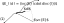
\includegraphics[width=0.25\textwidth]{img/2.png}
    %\caption{}
    %\label{fig:}
\end{figure}

\noindent
Из этих уравнений легко получить, что
\begin{equation}
    \left\{\begin{aligned}
        \frac{\partial U}{\partial z} &= - \frac{L_0}{c^2} \frac{d I}{d t} \\
        \frac{\partial I}{\partial z} &= - C_0 \frac{\partial U}{\partial t} 
    \end{aligned}\right.
    \hspace{0.5cm} \Rightarrow \hspace{0.5cm} 
    \boxed{
        \frac{\partial^2 U}{\partial t^2}  = \frac{c^2}{L_0 C_0} - \frac{\partial^2 V}{\partial z^2} 
    }.
\end{equation}
Решение аналогично будем искать в виде
\begin{equation}
    V = f_1 (z - vt) + f_2 (z + vt),
    \hspace{0.5cm} \Rightarrow \hspace{0.5cm} 
    v = \frac{c}{\sqrt{L_0 C_0}}.
\end{equation}
Кстати, если это всё посчитать для коаксиального кабеля, то
\begin{equation*}
    L_0 = 2 \mu \ln \frac{R_2}{R_1} , \hspace{0.5cm} 
    C_0 = \frac{\varepsilon}{2 \ln \frac{R_2}{R_1} },
    \hspace{0.5cm} \Rightarrow \hspace{0.5cm} 
    v = \frac{c}{\sqrt{\mu \varepsilon}}.
\end{equation*}


\subsubsection*{Коэффициент стоячей волны (standing wave ratio)}
Коэффициент стоячей волны -- отношение наибольшего значения амплитуды напряжённости электрического или магнитного поля стоячей волны в пучностях линии передачи к амплитуде в узлах.
КСВ является мерой согласования нагрузки (например, антенны) с линией передачи.

Наибольшее и наименьшее значения амплитуды соответсвенно равны
\begin{equation*}
    A_{\text{max}} = A_{\text{inc}} + A_{\text{ref}}, \hspace{0.5cm} 
    A_{\text{min}} = A_{\text{inc}} - A_{\text{ref}},
    \hspace{0.5cm} \Rightarrow \hspace{0.5cm} 
    \text{КСВ} = \frac{A_{\text{inc}} + A_{\text{ref}}}{A_{\text{inc}} - A_{\text{ref}}} = 
    \frac{1 + |\Gamma|}{1 - |\Gamma|},
\end{equation*}
где $|\Gamma|$ -- коэффициент отражения.

\subsubsection*{Согласованная нагрузка}
Рассмотрим длинную линию, пусть в цепи 
\begin{equation*}
    U = U_0 \cos \left(\omega_0 t - kz\right),  \hspace{0.5cm} 
    I = I_0 \cos \left(\omega_0 t - kz\right).
\end{equation*}
Сделаем следующий трюк. Возьмем, и продолжим линию до бесконечности, от которой, очевидно, ничего не отразится. Соотвественно нас интересует поиск эквивалентного импеданса системы. 
\begin{align*}
    U^* = U_0 \exp\left(i(\omega_0 t - kz)\right) &= U_0 e^{ikz} e^{-i\omega_0 t}, \\
    I^* = I_0 \exp\left(i(\omega_0 t - kz)\right) &= I_0 e^{ikz} e^{-i\omega_0 t}.
\end{align*}
Подставив эти выражения в волновое уравнение, и получим
\begin{equation*}
    ik U^* = i \omega_0 I^*,
    \hspace{0.5cm} 
    Z^* = U^* / I^* = \frac{\omega_0}{k},
    \hspace{0.5cm} \Rightarrow \hspace{0.5cm} 
    R = \frac{1}{c} \sqrt{\frac{L_0}{C_0}},
    \text{\ \ --- \ \ \textit{согласованная нагрузка}}.
\end{equation*}
То есть при наличии такого сопротивления на конце линии не будет никакого отражения. 




\sbsnum{25}{Элементы гидродинамики}
\subsubsection*{Уравнение непрерывности}
\begin{to_def}[Предмет рассмотрения]
	Ввиду макроскопического рассмотрения \textit{жидкости}(газы) в гидродинамике представлется как сплошная среда, то есть малый элемент объёма жидкости содержит ещё достаточно больше количество молекул, относительно межмолекулярного расстояния.
\end{to_def}

Для описания движения жидкости требуется задать распределение скорости жидкости $\vc{v} = \vc{v}(x,y,z,t)$ и какие-либо её две термодинамические величины, как, например, плотность и давление. Важно отметить, что все эти величины относятся не к отдельной частице, а к точке в пространстве в определенное время.

\begin{to_thr}[Уравнение непрерывности]
\phantom{239}

\begin{proof}[$\triangle$]
	В маленьком объёме $V_{0}$ количество жидкости есть $\int_{V_0} \rho d V$.
	Через элемент поверхности, ограничивающей $V_0$, в единицу времени протекает $\rho \vc{v} \cdot d \vc{f}$ жидкости --- положительно или отрицательное число, в зависимости от того, вытекает или втекает жидкость соответственно.
	Тогда приравниваем для вытекания жидкости два наших рассуждения:
	\begin{equation*}
		- \frac{\partial}{\partial t} \int \rho d V =  \oint \rho \vc{v} \cdot d \vc{f}
		\hspace*{0.5 cm} 
		\Rightarrow 
		\hspace*{0.5 cm}
		\int \left(\frac{\partial \rho}{\partial t} + \div \rho \vc{v}\right)d V = 0
		\hspace*{0.5 cm}
		\Rightarrow
		\hspace*{0.5 cm}
		\frac{\partial \rho}{\partial t} + \div \rho \vc{v} = 0.
	\end{equation*}
	Последнее следует из того, что равенство должно иметь для любого объёма, таким образом получили искомое \textit{уравнение непрерывности}.
\end{proof}
	
\end{to_thr}

\subsubsection*{Уравнение Эйлера}

\begin{to_thr}[Уравнение Эйлера]
\phantom{239}

\begin{proof}[$\triangle$]
	Выделим в жидкости некоторый объём, полная сила, действующая на этот объём: $- \oint p d \vc{f} = - \int \grad p d V$, где интеграл из взятого по поверхности объёма преобразуется в сам рассматриваемый объём.
	Таким образом получили, что на единицу объёма жидкости будет действовать сила:
	\begin{equation*}
		\rho \frac{d \vc{v}}{d t} = - \grad p.
	\end{equation*}
	Однако стоящая здесь скорость определяет изменение скорости именно элемента объёма, а не точки в пространстве.
	Запишем это изменение скорости:
	\begin{equation*}
		d \vc{v} 
		=
		 \frac{\partial \vc{v}}{\partial t} d t + \frac{\partial \vc{v}}{\partial x^i} d x^i 
		= 
		\frac{\partial \vc{v}}{\partial t} d t + (d \vc{r} \cdot \nabla) \vc{v}
		\hspace*{1 cm}
		\Rightarrow
		\hspace*{1 cm}
		\frac{\partial \vc{v}}{\partial t} + (\vc{v} \nabla) \vc{v} = - \frac{1}{\rho} \grad p.
	\end{equation*}
	Последнее и есть искомое уравнение Эйлера.
\end{proof}
\end{to_thr}

Если же жидкость движется во внешнем поле тяжести, то, на каждый элемент объёма будет действовать сила, которая просто добавится к изначальному уравнению: 
\begin{equation*}
	\frac{\partial \vc{v}}{\partial t} + (\vc{v} \nabla) \vc{v} = - \frac{\nabla p}{\rho} + \vc{g}.
\end{equation*}

\subsubsection*{Уравнение Навье-Стокса}

Чтобы нормально учесть вязкость, нужно поговорить про \textit{поток импульса}.
Импульс единицы объёма жидкости есть $\rho \vc{v}$, скорость изменения его компоненты:
\begin{equation*}
	\frac{\partial}{\partial t} \rho v^i = \rho \frac{\partial v^i}{\partial t} + \frac{\partial \rho}{\partial t} v^i.
\end{equation*}
Уравнения непрерывности и Эйлера запишутся в тензорном виде:
\begin{equation*}
	\frac{\partial \rho}{\partial t} = - \frac{\partial (\rho v^k)}{\partial x^k},
	\hspace*{0.5 cm}
	\hspace*{0.5 cm}
	\frac{\partial v^i}{\partial t} = - v^k \frac{\partial v^i}{\partial x^k} - \frac{1}{\rho} \delta^{i k} \frac{\partial p}{\partial x^k}.
\end{equation*}
Тогда получим:
\begin{equation*}
	\frac{\partial}{\partial t} \rho v^i 
	= 
	- \rho v^k \frac{\partial v^i}{\partial x^k} -  \delta^{i k} \frac{\partial p}{\partial x^k} - v^i \frac{\partial \rho v^k}{\partial x^k} 
	=
	-\delta^{i k} \frac{\partial p}{\partial x^k} - \frac{\partial}{\partial x^k} \rho v^i v^k
	= - \frac{\partial \Pi^{i k}}{\partial x^k}.
\end{equation*}
\begin{to_def}
	$\Pi^{i k} $ --- \textit{тензор плотности потока импульса}:
	$
		\Pi^{i k} = p \delta^{i k} + \rho v^i v^k.
	$
\end{to_def}

Таким образом уравнение Эйлера у нас записалось в виде:
$
	\frac{\partial}{\partial t} \rho v^i = - \frac{\partial \Pi^{i k}}{\partial x^k}.
$
Поток импульса представляет собой чисто обратимый перенос импульса, связанный с просто механическим передвижением различных участков жидкости и с действующими в жидкости силами давления.
\textit{Вязкость} (внутреннее трение) жидкости проявляется в наличии ещё дополнительного, необратимого переноса импульса из мест с большой скоростью в места с меньшей.

Поэтому уравнение движения вязкой жидкости можно получить, прибавив к идеальному потоку импульса дополнительный член $\sigma^{i k}_{visc}$, определяющий такой вязкий перенос:
$
\Pi^{i k} = p \delta^{i k} + \rho v^i v^k - \sigma^{i k}_{visc} = - \sigma^{i k} + \rho v^i v^k.
$
\begin{to_def}
	Таким образом: $\sigma^{i k} = - p \delta^{i k} + \sigma^{i k}_{visc}$ называют \textit{тензором напряжений}, а $\sigma^{i k}_{visc}$ --- вязким тензором напряжений.
\end{to_def}

Чтобы написать выражение для вязкого напряжения сделаем пару оговорок. 
\textit{Во первых}, градиенты скорости движения участков жидкости относительно друг друга не велики, тогда $\sigma^{i k}_{visc}$ зависит лишь от первых производных скорости по координатам, линейно. \textit{Во вторых}, не зависящие от первых производных величины должны обращаться в нуль как для скорости потока $\vc{v} = \const$ и тензор должен быть нулевым. \textit{В третьих}, $\sigma^{i k}_{visc} = 0$ когда жидкость совершает целое равномерное вращение, поскольку никакого внутреннего трения тогда не будет.
Для такого равномерного вращения с $\vc{v} = [\vc{\omega} \vc{r}]$ линейными комбинациями производных обращающимися в нуль будут: $\frac{\partial v^i}{\partial x^k} + \frac{\partial v^k}{\partial x^i}$.

Это всё даёт нам мотивацию для не шибко сильных потоков несжимаемой жидкости согласится с Сэром Исааком Ньютоном, и написать тензор вязкого напряжения, как \textit{тензор скорости деформации}:
\begin{equation*}
	\sigma^{i k}_{visc} = \eta \left(\frac{\partial v^i}{\partial x^k} + \frac{\partial v^k}{\partial x^i}\right),
	\hspace*{1 cm}
	\Rightarrow
	\hspace*{1 cm}
	\sigma^{i k} = - p \delta^{i k} + \eta \left(\frac{\partial v^i}{\partial x^k} + \frac{\partial v^k}{\partial x^i}\right).
\end{equation*}
А уравнение Эйлера тогда для несжимаемой жидкости запишется:
\begin{equation*}
	\rho \left(\frac{\partial v^i}{\partial t} + v^k \frac{\partial v^i}{\partial x^k}\right)
	=
	- \delta^{i k} \frac{\partial p}{\partial x^k} + \frac{\partial}{\partial x^k} \left[\eta \left(\frac{\partial v^i}{\partial x^k} + \frac{\partial v^k}{\partial x^i}\right)\right].
\end{equation*}
а в более человеческом, привычном глазу, виде \textit{уравнение Навье-Стокса для несжимаемой жидкости}:
\begin{equation*}
	\frac{\partial \vc{v}}{\partial t} + (\vc{v} \triangle) \vc{v} = - \frac{1}{\rho} \grad p + \frac{\eta}{\rho} \Delta \vc{v}.
\end{equation*}
\begin{to_def}
	Коэффициент $\eta$ называется --- \textit{динамическим коэффициентом вязкости}, а отношение $\eta/\rho = \nu$ --- \textit{кинематической вязкостью}.
\end{to_def}



%%%%%%%%%%%%%%%%%%%%%%%%%%%%%%%%%%%%%%%%%%%%%%%%%%%%%%%%%%%%%%%%%%%%%%%%%%%%%%%%%%%
\secnum{6}{Принципиальность виртуальных перемещений} % 26-30
%%%%%%%%%%%%%%%%%%%%%%%%%%%%%%%%%%%%%%%%%%%%%%%%%%%%%%%%%%%%%%%%%%%%%%%%%%%%%%%%%%%


\sbsnum{28}{(вплоть до №30) Общее уравнение динамики, статики и т.д.}

Легко получить соотношение вида
\begin{equation}
    \sum_{i=1}^N \left(
        \vc{F}_i - m_i \vc{\mathrm{w}}_i
    \right) \cdot \delta \vc{r}_i = 0.
\end{equation}
Данное соотношение является необходимым и достаточным условием для того, чтобы движение, совместимое с идеальными связями, отвечало данной системе активных сил $\vc{F}_i$. Оно получило название \textbf{общего уравнения динамики} или \textit{дифференциальным вариационным принципом Даламбера-Лагранжа}.

\begin{to_thr} [принцип Даламбера-Лагранжа]
Верно, что
\begin{equation*}
    m_i \vc{\mathrm{w}}_i = \vc{F}_i + \vc{R}_i,
    \hspace{0.5cm} \Rightarrow \hspace{0.5cm} 
    \sum_i \left(
       \vc{F}_i -  m_i \vc{\mathrm{w}}_i
    \right) \cdot \delta \vc{r}_i = 0.
\end{equation*}
\end{to_thr}

Аналогично можно сформулировать \textit{принцип Журдена}
\begin{equation}
    \sum_{i=1}^N \left(
        \vc{F}_i - m_q \vc{\mathrm{w}}_i
    \right) \cdot \delta  \vc{v}_i = 0,
\end{equation}
и \textit{принцип Гаусса}:
\begin{equation}
    \sum_{i=1}^N \left(
        \vc{F}_i - m_q \vc{\mathrm{w}}_i
    \right) \cdot \delta \vc{\mathrm{w}}_i = 0,
\end{equation}
где $\delta \vc{\mathrm{w}}_i = \vc{\mathrm{w}}^*_{i_1} - \vc{\mathrm{w}}^*_{i_2}$ не обязательно малая величина. 

Замечая, что $m_i = \const$, а $\vc{F}_i = \vc{F}_i (p, q)$, то последнее уравнение перепишется в виде
\begin{equation*}
    Z = \frac{1}{2} \sum_{i=1}^N m_i 
    \left(
        \vc{\mathrm{w}}_i - \frac{\vc{F}_i}{m_i} 
    \right)^2,
    \hspace{1cm} 
    \delta Z = 0,
\end{equation*}
где величина $Z$ называется принуждением или мерой принуждения. К слову она не просто стационарна для истинных движений. 

\texttt{Истинным является движение с минимальной мерой принуждения.} Другими словами \textit{несвободная система совершает движение, наиболее близкое к свободному}. 

\begin{to_def} 
    Будем считать, что $q^0 \in M$ -- \textit{точка равновесия}, если при $\dot{q}^0 \equiv \dot{q}(0) \equiv 0$ приводит к $q(t) = q^0$. 
\end{to_def}

В таком случае верен следующий принцип:

\begin{to_thr}[принцип Лагранжа]
    Для того, чтобы точка была положением равновесия на $t \in [t_1, t_2]$ необходимо и достаточно, чтобы сумма элементарных работ на $\forall$ виртуальных перемещениях всех активных сил была равна нулю.
    \begin{equation}
        \delta A \big|_0 = 0 
        \hspace{0.5cm} 
        \delta A = \sum_i \vc{F}_i \cdot \delta \vc{r}_i,
        \hspace{0.5cm} (t\in[t_1, t_2])
    \end{equation}
    что является \textbf{общим уравнением статики}.
\end{to_thr}

Этот принцип можно рассматривать, как дракона с тремя головами. Вот если система \textbf{голономная}, то
\begin{equation*}
    \delta A = Q_i \delta q_i 
    \hspace{0.5cm} \Rightarrow \hspace{0.5cm} 
    Q_i = 0 \ \forall i.
\end{equation*}
Если система \textbf{консервативная}, то
\begin{equation*}
    Q_1 = - \frac{\partial P}{\partial q^i} 
    \hspace{0.5cm} \Rightarrow \hspace{0.5cm} 
    \text{положение равновесия --- стационарная точка потенциала}.
\end{equation*}
Если же у нас \textbf{твёрдое тело}, тогда
\begin{equation*}
    \delta A = \left(
        \vc{R}^{\text{внеш}} \cdot \vc{v}_O
    \right) \d t + 
    \left(
        \vc{M}_O^{\text{внеш}} \cdot \vc{\omega}
    \right) dt
    \hspace{0.5cm} \Rightarrow \hspace{0.5cm} 
    \left\{\begin{aligned}
        \vc{R}^{\text{внеш}} &= 0 \\
        \vc{M}^{\text{внеш}} &= 0 \\
    \end{aligned}\right.
\end{equation*}




%%%%%%%%%%%%%%%%%%%%%%%%%%%%%%%%%%%%%%%%%%%%%%%%%%%%%%%%%%%%%%%%%%%%%%%%%%%%%%%%%%%
\secnum{7}{Уравнения Лагранжа} % 31-34
%%%%%%%%%%%%%%%%%%%%%%%%%%%%%%%%%%%%%%%%%%%%%%%%%%%%%%%%%%%%%%%%%%%%%%%%%%%%%%%%%%%

\sbsnum{31}{Уравнение Лагранжа второго рода}
\begin{to_lem}[Разбиение единицы в окрестности компакта на многообразии]
     Пусть $M$ -- гладкое многообразие, а $K \subseteq M$ -- его компактное подмножество. Для любого покрытия $\{U_\alpha\}_\alpha$ компакта $K$ открытыми множествами найдётся набор неотрицательных гладких функций $\{\rho_\alpha\}_\alpha$ с компактными носителями $\mathrm{supp}\, \rho_\alpha$ таких, что
\begin{equation*}
    \forall \alpha \ \textnormal{supp}\, \rho_\alpha \subset U_\alpha,
\end{equation*}
    только конечное число из них отлично от нуля и
    $\sum_\alpha \rho_\alpha (x) \equiv 1$
    в некоторой окрестности $K$.
\end{to_lem}

\begin{to_def} 
    Интеграл дифференциальной формы $\nu \in \Omega_{\text{c}}^n (M)$ с компактным носителем по ориентированному $n$-мерному многообразию $M$ определяется с помощью разбиения единицы в окрестности носителя $\nu$ 
    \begin{equation*}
         \rho_1 + \ldots + \rho_m = 1,
     \end{equation*} 
     подчиненного некоторому набору положительно ориентрированных карт как
     \begin{equation*}
         \int_M \nu = \sum_i \int_M \rho_i \nu_i,
     \end{equation*}
     где интегралы справа рассматриваются в координатных картах, содержащих носители соответствующих $\rho_i$.
\end{to_def}

\begin{to_lem} 
    Определение интеграла не зависит от выбора системы положительных карт в данной ориентации и подчиненного им разбиения единциы. 
\end{to_lem}





\sbsnum{32}{Разрешимость уравнений Лагранжа}
Подставим разложение кинетической энергии в уравнения Лагранжа, оставив только слагаемые с обобщёнными ускорениями $f_j (q, \dot{q}, t) = a_{jk} \ddot{q}^j$. 
\begin{equation*}
    T = \frac{1}{2} \sum_\nu m_\nu \dot{\vc{r}}_\nu^2 = \frac{1}{2} \sum_\nu
    \left(
        \frac{\partial \vc{r}_\nu}{\partial q^j} \dot{q}^j + \frac{\partial \vc{r}_\nu}{\partial t} 
    \right)^2 = 
    \frac{1}{2} 
    \bigg[
    \underbrace{
        a_{jk} \dot{q}^j \dot{q}^k
    }_{
        2T_2
    } +
    \underbrace{
        a_j \dot{q}^j
    }_{
        2T_1
    } +
    \underbrace{
        a_0
    }_{
        2T_0
    }
    \bigg],
\end{equation*}
где коэффициенты, соответственно, равны 
\begin{equation*}
    a_{jk}(q, t) = \sum_\nu m_\nu \frac{\partial \vc{r}_\nu}{\partial q^j} \cdot \frac{\partial \vc{r}_\nu}{\partial q^k},
    \hspace{0.5cm} 
    a_j(q, t) = \sum_\nu m_\nu \frac{\partial \vc{r}_\nu}{\partial q^j} \cdot \frac{\partial \vc{r}_\nu}{\partial t},
    \hspace{0.5cm} 
    a_0 = \sum_\nu m_\nu 
    \left(
    \frac{\partial \vc{r}_\nu}{\partial t} 
            \right)^2.
\end{equation*}
Для склерономных систем $\partial \vc{r}_\nu / \partial t = 0$, соотвественно $T = a_{jk} \dot{q}^j \dot{q}^k$, при чём $a_{jk} \equiv a_{jk} (q)$.

Теперь подставим значение $T$ в уравнения Лагранжа, и получим, что
$
    a_{ik} \ddot{q}^k = f_i,
$
где $f_1 = f_1(q, \dot{q}, t)$. Уравнений в системе $n$, причём $a_{jk}$ является положительно определенной формой\footnote{
    \red{Требует отдельного доказательства.}
}, соответственно невырожденной. 

\begin{to_thr} 
    Уравнения Лагранжа второго рода разрешимы относительно обобщенных ускорений 
\end{to_thr}


\sbsnum{37}{Ковариантность уравнений Лагранжа}
\begin{to_tas}
	Для не обязательно компактного многообразия без края $M$ рассмотрим дифференциальные формы с компактным носителем $\Omega_c^*(M)$ и определим когомологии де Рама с компактным носителем:
	\begin{equation*}
		H_c^k (M) = \left(ker d \colon \Omega_c^k (M) \rightarrow \Omega^{k+1}_c (M)\right) / \Im \d \colon \Omega_c^{k-1}(M) \rightarrow \Omega_c^{k}(M).
	\end{equation*}

	Если $ \dim M = n$, M ориентируемо и связно, \textbf{то} $H_c^n(M)$ одномерно.
\end{to_tas}

\begin{to_tas}
	$H_c^k (\mathbb{R}^n) = 0$ при $k \neq n$, и $H_c^n(\mathbb{R}^n) = \mathbb{R} $.
\end{to_tas}

\sbsnum{33}{Изменение полной мехнической энергии голономной системы}
 % \renewcommand{\labelenumi}{\Roman{enumii}}
\begin{enumerate}[label={$\mathbb{R}^\text{\arabic*}$.}]
    \item Формула Стокса для ориентированной кривой с началом в точке $p$ и концом в точке $q$ сводится к 
    \begin{equation*}
        \int_\gamma \d f = f(q) - f(p).
    \end{equation*}
    \item Для компактного множества $G \subset \mathbb{R}^2$ с гладкой границей, ориентированного так, что при движении по $\partial G$ множество $G$ оказывается слева, верна \textit{формула Грина}
    \begin{equation*}
        \int_{\partial G} P \d x + Q \d y = \int_G
        \left(
            \frac{\partial Q}{\partial x} - \frac{\partial P}{\partial y} 
        \right) \d x \wedge d y.
    \end{equation*}
    \item Для компактного множества $G \subset \mathbb{R}^3$ с гладкой границей (край в $\mathbb{R}^3$) верна \textit{формула Гаусса-Остроградского}
    \begin{equation*}
        \int_{\partial G} P \d y \wedge d z 
        + Q \d z \wedge dx 
        + R \d x \wedge dy = 
        \int_G
        \left(
            \frac{\partial P}{\partial x} +
            \frac{\partial Q}{\partial y} +
            \frac{\partial R}{\partial z} 
        \right) \d x \wedge d y \wedge d z.
    \end{equation*}
\end{enumerate}


Кривую можно считать не бесконечно гладкой, а всего лишь кусочно непрерывно дифференцируемой, формула всё равно остаётся верной. С помощью предельного перехода также обобщается случай с $\simeq \mathbb{R}^2$ до множества с кусочно $C^2$ границей.

Вообще формула Стокса верна не только для вложенных двумерных многообразий, но и для всякого образа гладкого отображения $f \colon D \mapsto  \mathbb{R}^3$ области $D \subset \mathbb{R}^2$ с кусочно гладкой границей, если интегралы мы понимаем как интегралы обратных образов $f^*(\alpha)$ и $f^*(d\alpha)$ по $\partial D$ и $D$ соответственно. Для практических применений полезно ослабить условие гладкости $f$ до $C^2$ (в интеграле, в координатном представлении, используются производные $f$ не более чем первого порядка).


% Кривую 



\sbsnum{34}{Обобщенный потенциал и первые интегралы лагранжевых систем}
Физический потенциал силового поля в математический терминах означает поиск $f \in C^\infty (M) \colon \d f = \alpha$ для заданной силы $\alpha \in \Omega^1(M)$

\begin{to_thr}
	Необходимым и достаточным условием наличия потенциала у непрерывной $\alpha \in \Omega^1(M)$, для гладкого $M$, является независимость $\int_\gamma \alpha$ от выбора между двумя точками кусочно-гладкой кривой $\gamma$.

	Эквивалентно можно потребовать равенства нулю интегралов по всем замкнутым кусочно-гладким кривым.
	\label{thr_7.1}
\end{to_thr}

Удобным на практике необходимым условием существования потенциала у $\alpha \in \Omega^1(M)$ является $\d \alpha = 0$ (т.к. $\d (\d u) = 0$).
Однако этого не достаточно, так например в открытой $U = \mathbb{R}^2 \backslash \{ 0 \}$:
\begin{equation*}
	\alpha = \frac{x \d y - y \d x}{x^2 + y^2}
	\hspace*{0.5 cm} \leadsto \hspace*{0.5 cm}
	\d \alpha = 0,
	\hspace*{0.5 cm} \text{ но } \hspace*{0.5 cm}
	\oint_{S^1} \alpha = 2 \pi.
\end{equation*}

Далее в качестве упражнений оставлены следующие важные замечания:

\begin{to_tas}[Порядок точки относительно кривой]
Для замкнутой кусочно-гладкой $\gamma \in \mathbb{R}^2$, не проходящей через начало координат определим порядок начала координат относительно кривой:
\begin{equation*}
	w (\gamma, 0) - \frac{1}{2 \pi} \int_{\gamma} \frac{x \d y - y \d x}{x^2 + y^2},
\end{equation*}
и он не меняется при непрерывных деформациях кривой, при которых она не проходит через начало координат.
\end{to_tas}

\begin{to_tas}
	Порядок начала координат относительно кривой является целым.
\end{to_tas}

\begin{to_tas}
	Порядок начала координат относительно не проходящей через него нечётной кривой является нечётным числом. ($\gamma \colon \mathbb{S}^1 \rightarrow \mathbb{R}^2, \; \gamma(-u) = - \gamma(u)$).
\end{to_tas}

\begin{to_tas}
	Для замкнутой кривой на плоскости с всюду не нулевой скоростью $\int k(s) \d s = 2 \pi N, \; N \in \mathbb{Z}$.
\end{to_tas}

\begin{to_tas}[Лемма Жордана]
	Замкнутая кусочно-гладкая кривая $\gamma \subset \mathbb{R}^2$ без самопересечений делит плоскость на две связные части внутреннюю и внешнюю (можно усложнить и сформулировать для непрерывных кривых).
\end{to_tas}



%%%%%%%%%%%%%%%%%%%%%%%%%%%%%%%%%%%%%%%%%%%%%%%%%%%%%%%%%%%%%%%%%%%%%%%%%%%%%%%%%%%
\secnum{8}{Канонические уравнения} % 35-41 \ 38-39
%%%%%%%%%%%%%%%%%%%%%%%%%%%%%%%%%%%%%%%%%%%%%%%%%%%%%%%%%%%%%%%%%%%%%%%%%%%%%%%%%%%

\sbsnum{35}{Гамильтонов формализм, уравнения и интеграл Якоби}
\subsubsection*{Преобразование Лежандра}

\begin{to_def} 
    В уравнениях Лагранжа второго рода движения голономной системы в потенциальном поле сил, функция Лагранжа зависит от $q, \ \dot{q}, \ t$ -- \textit{переменные Лагранжа}.
    Если в качестве параметров взять $q, \ p, \ t$, где $p_i$ -- \textit{обобщенные импульсы}\footnote{
        Обобщенный импульс $p_i$ -- ковектор, а  не вектор!
    }, определяемые как
    $
        p_i = {\partial L}/{\partial \dot{q}^i}.
    $
    То получим набор $q, \ p, \ t$ -- \textit{переменные Гамильтона}. 
\end{to_def}

В силу невырожденности $\partial L / (\partial \dot{q}^i \partial \dot{q}^j) = J_{p}$, то есть по \textit{теореме о неявной функции} эти равенства разрешимы относительно переменных $\dot{q}^i$. Через преобразование Лежандра естестественно ввести функцию
\begin{equation*}
    H(q, p, t) = p_i \dot{q}^i - L(q, \dot{q}, t),  \hspace{0.5cm} \dot{q} \equiv \dot{q}(q, p, t).
\end{equation*}

\subsubsection*{Уравнения Гамильтона}
% Маркеев, п.149.

Полный дифференциал функции Гамильтона можем выразиь двумя способами:
\begin{equation*}
    \left.\begin{aligned}
        d H &= \frac{\partial H}{\partial q^i} \d q^i + \frac{\partial H}{\partial p_i} \d p_i + \frac{\partial H}{\partial t} \d t,
        \\
        dH &= \dot{q}^i \d p_i - \frac{\partial L}{\partial q^i} \d q^i - \frac{\partial L}{\partial t} \d t.
    \end{aligned}\right\}
    \hspace{0.7cm} \Rightarrow \hspace{0.7cm} 
    \left.\begin{gathered}
        \frac{\partial H}{\partial t} = - \frac{\partial L}{\partial t} \\
        \frac{\partial H}{\partial p_i} = \dot{q}^i, \ \ 
        \frac{\partial H}{\partial q^i} = - \frac{\partial L}{\partial q^i}
    \end{gathered}\right.
    \hspace{0.7cm} \Rightarrow \hspace{0.7cm} 
    \left\{\begin{aligned}
        \frac{d q^i}{d t} &= \frac{\partial H}{\partial p_i}, \\
        \frac{d p_i}{d t} &= - \frac{\partial H}{\partial q^i}.    
    \end{aligned}\right.
\end{equation*}
Эти уравнения называются \textit{уравнениями Гамильтона}, или \textit{каноническими уравнениями}.


\subsubsection*{Физический смысл функции Гамильтона}

Пусть система натуральна, тогда $L = L_2 + L_1 + L_0$, и, соответсвенно,
\begin{equation*}
    H = \frac{\partial L}{\partial \dot{q}^i} \dot{q}^i - L.
\end{equation*}
По теореме Эйлера об однородных функциях
\begin{equation*}
    \frac{\partial L_2}{\partial \dot{q}^i} \dot{q}^i = 2 L_2,
    \hspace{1cm} 
    \frac{\partial L_1}{\partial \dot{q}^i} \dot{q}^i = L_1,
    \hspace{0.5cm} \Rightarrow \hspace{0.5cm} 
    H = L_2 - L_0.
\end{equation*}
пусть $T = T_2 + T_1 + T_0$, если силы имеют обычный потенциал $\Pi$, то $L_0 = T_0 - \Pi$, 
\begin{equation*}
    H = T_2 - T_0 + \Pi.
\end{equation*}
Если же силы имеют обобщенный потенциал $V = V_1 + V_0$, то $L_0 = T_0 - V_0$, и
\begin{equation*}
    H = T_2 - T_0 + V_0.
\end{equation*}
В случае натуральных и склерономных систем $T_1 = T_0 = 0$ и $T = T_2$, тогда $H = T + \Pi$. Т.е. для натуральных склерономных систем с обычным потенциалом сил функция Гамильтона $H$ представляет собой полную механическую энергию.

\subsubsection*{Интеграл Якоби}

Найдём полную производную $H$ по времени,
\begin{equation*}
    \frac{d H}{d t} = \frac{\partial H}{\partial q^i} \dot{q}^i + \frac{\partial H}{\partial p_i} \dot{p}_i + \frac{\partial h}{\partial t} = 
    \frac{\partial H}{\partial q^i} \frac{\partial H}{\partial p_i} - \frac{\partial H}{\partial p_i} \frac{\partial H}{\partial q^i} + \frac{\partial H}{\partial t} = \frac{\partial H}{\partial t},
    \hspace{0.5cm} \Rightarrow \hspace{0.5cm} 
    \frac{d H}{d t} = \frac{\partial h}{\partial t}.
\end{equation*}
Система называется \textit{обобщенно консервативной}, если $\partial H / \partial t = 0$, т.е $H(q^i, p_i) = h$, собственно, $H$ называют \textit{обобщенной полной энергией}, а поледнее равенство -- \textit{обобщенным интегралом энергии}.


\begin{to_def} 
    Для натуральной системы с обычным потенциалом сил, если $\partial H/ \partial t =0$, то
    \begin{equation*}
         H = T_2 - T_0 + \Pi = h = \const.
     \end{equation*} 
     Соотноешние, где $h$ -- произвольная постоянная, называют \textit{интегралом Якоби}.
\end{to_def}

Есть и другая формулировка для интеграла Якоби голономной склерономной системы. Действительно, при $\partial L / \partial t = 0$, интеграл Якоби перейдёт в
\begin{equation*}
    \frac{\partial H}{\partial t} = 0,
    \hspace{0.25cm} \Rightarrow \hspace{0.25cm} 
    \frac{d }{d t} \left(
        \frac{\partial L}{\partial \dot{q}^i} \dot{q}^i
    \right) = 0,
    \hspace{0.25cm} \Rightarrow \hspace{0.25cm} 
    \frac{\partial L}{\partial \dot{q}^i} \dot{q}^i = \const.
\end{equation*}



\subsubsection*{Уравнения Уиттекера}


Если $\partial H / \partial t = 0$, то $H(q, p) = h$, где $h = \const$ определяемая из н.у. В $2n$-мерном пространстве $q, \ p$ интеграл Якобми задаёт гиперповерхность, рассмотрим движение с $H = h$.

Такое движение описывается системой с $2n-2$ уравнений, причём она может быть записана в виде канонических уравнений. Пусть $\partial H / \partial p_1 \neq 0$, тогда
\begin{equation*}
    p_1 = - K(q^1, \ldots, q^n, p_2, \ldots, p_n, h),
    \hspace{0.5cm} \Rightarrow \hspace{0.5cm} 
    \left\{\begin{aligned}
        \dot{q}^i = \frac{\partial H}{\partial p_i}, \\
        \dot{p}_j = - \frac{\partial H}{\partial q^j}        
    \end{aligned}\right.
    \hspace{0.5cm} \Rightarrow \hspace{0.5cm} 
    \frac{d q^j}{d q^1} = \frac{
    \left(\dfrac{\partial H}{\partial p_j} \right)
    }{
    \left(\dfrac{\partial H}{\partial p_1} \right)
    },
    \hspace{0.5cm} 
    \frac{d p_j}{d q^1} = - \frac{
    \left(\dfrac{\partial H}{\partial q^j}\right)
    }{
    \left(\dfrac{\partial H}{\partial p_1} \right)
    },
\end{equation*}
для $j = 2,\ 3,\ \ldots,\ n$. Подставляя $p_1$ получим
\begin{align*}
    &\frac{\partial H}{\partial q^j} - \frac{\partial H}{\partial p_1} \frac{\partial K}{\partial q^j} = 0,
    &(j = 2, \ 3, \ \ldots, n);
    \\
    &\frac{\partial H}{\partial p_j} - \frac{\partial H}{\partial p_1} \frac{\partial K}{\partial p_j}  = 0,
    &(j = 2, \ 3, \ \ldots, n).
\end{align*}
Допиливая до надлежащего вида, окончательно находим
\begin{equation*}
    \frac{d q^j}{d q^1} = \frac{\partial K}{\partial p_j},
    \hspace{1cm} 
    \frac{d p_j}{d q_1} = - \frac{\partial K}{\partial q^j},
    \hspace{1cm} 
    (j = 2, \ 3, \ \ldots, n).
\end{equation*}
Эти уравнения описывают движения системы при $H = h = \const$, и называются \textit{уравнениями Уиттекера}. 

\subsubsection*{Уравнения Якоби}


Уравнения Уиттекера имеют структуру уравнений Гамильтона, соответственно их можно зписать в виде уравнений типа Лагранжа, при гессиане $K$ по $p$ неравным 0. Пусть $P$ -- преобразование Лежандра функции $K$ по $p_j$ ($j = 2, \ 3,\ \ldots,\ n$). Тогда
\begin{equation*}
    P = P(q^2, \ldots, q^n, \tilde q^2, \ldots, \tilde q^n, q^1, h) = \sum_{j = 2}^{n} \tilde q^j p_j - K,
\end{equation*}
где $\tilde q^{j} = d q^j / d q^1$. Величины $p_j$ выражаются через $\tilde q^2, \ \ldots, \ \tilde q_n$ из уравнений 
\begin{equation*}
    \tilde q^j = \frac{\partial K}{\partial p_j}, \hspace{0.5cm} 
    (j = 2, \ 3, \ \ldots, n),
\end{equation*}
т.е. из первых $n-1$ уравнений Уиттекера. При помощи функции $P$ эти уравнения могут быть записаны в эквивалентной форме:
\begin{equation*}
    \frac{d }{d q^1} \frac{\partial P}{\partial q_j'} - \frac{\partial P}{\partial q^j} = 0
    \hspace{1cm} (j = 2,\ 3,\ \ldots,\ n).
\end{equation*}
Это уравнения типа Лагранжа, называются \textit{уравнениями Якоби}.

Преобразовывая выражение для $P$ найдём, что
\begin{equation*}
    P = \sum_{j=2}^{n} q_j \tilde q^j + p_1 = 
    \sum_{i=1}^{n} p_1 \tilde q_i = \frac{1}{\dot{q}^1} \sum_{i=1}^{n} p_i \dot{q}^i = \frac{1}{\dot{q}^1} (L+H).
\end{equation*}
Тогда в случае консервативной системы $L = T - \Pi$, $H = T + \Pi$, и\footnote{
    \red{Пара выражений в выводе опущены.}
}
\begin{equation*}
    P = \frac{2T}{\dot{q}^1},
    \hspace{0.5cm} \Rightarrow \hspace{0.5cm} 
    P = 2 \sqrt{(h-\Pi) G}.
\end{equation*}



\sbsnum{36}{Принцип наименьшего действия}
\subsubsection*{Пара слов от Льва Давидовича}


\begin{to_def} 
    \textit{Действием по Гамильтону} называют функционал вида
    \begin{equation*}
         S = \int_{t_0}^{t_1} L(\gamma(t), \dot{\gamma}(t), t) \d t.
    \end{equation*} 
    Переходя к однопараметрическому семейству кривых $\gamma(\alpha, t)$ получим \textit{вариацию действия}
    \begin{equation*}
        S = \int_{t_0}^{t_1} L(\gamma(\alpha, t), \dot{\gamma}(\alpha, t), t) \d t, 
        \hspace{0.5cm} 
        \delta S = \frac{d S}{d \alpha} \delta \alpha.
    \end{equation*}
\end{to_def}


\begin{to_thr}[принцип Гамильтона]
    Кривая $\gamma(\alpha, t)$ является экстремалью действия тогда и только тогда, когда является решением уравнений Лагранжа
     \begin{equation*}
         \delta S = 0
         \hspace{0.5cm} \Leftrightarrow \hspace{0.5cm} 
         \gamma(\alpha, t) \in \textnormal{Sol}\,
         \left(
     \frac{d}{dt} \frac{\partial L}{\partial \dot{q}^k} - \frac{\partial L}{\partial q^k} = 0
         \right)
         .
     \end{equation*}
\end{to_thr}


\begin{proof}[$\triangle$]
    Давайте просто проварьируем Лагранжиан, тогда
    \begin{align*}
        \delta S 
        &=
         \int_{t_0}^{t_1} 
        \left(
            \frac{\partial L}{\partial q^i} \frac{\partial q^i}{\partial \alpha} +
            \frac{\partial L}{\partial \dot{q}^i} \frac{\partial \dot{q}^i}{\partial \alpha}  
        \right) \delta \alpha \d t 
        =
        \int_{t_0}^{t_1} \left(
            \frac{\partial L}{\partial q^i} \delta q^i + \frac{\partial L}{\partial \dot{q}^i} \delta \dot{q}^i
        \right) \d t
        =
        \frac{\partial L}{\partial \dot{q}} \partial q \bigg|_{t_1}^{t_2}
        + \int_{t_1}^{t_2}
        \left(
            \frac{\partial L}{\partial q^i} - \frac{d }{d t} \frac{\partial L}{\partial \dot{q}^i} 
        \right) \,\delta q^i \d t
        = 0.
    \end{align*}
    таким образом уравнения Лагранжа выполнены. 
\end{proof}


\subsubsection*{Истинные и окольные пути}

\begin{to_def} 
    Совокупность траекторий, которые описаны перемещениями из начальных положений $a_\nu$ в конечные $b_\nu$, образуют \textit{истинный} (\textit{действительный, прямой}) путь системы $\gamma_\nu$.

    Совокупность $\gamma_\nu'$, бесконечно близких к $\gamma_\nu$ и таких, что движение точки по кривой $\gamma_\nu'$ может происходить без нарушения связей, называют окольным путем системы.
\end{to_def}

\begin{to_def} 
    \textit{Расширенное координатным пространство} помимо криволинейных координат $q^i$ также время $t$.
\end{to_def}

\begin{to_def} 
    При достаточном удалении точки $A_1$ от точки $A_0$ может оказаться, что краевая задача имеет решения, соответствующие бесконечно близким прямым путям в расширенном координатном пространстве. В этом случае точки $A_0$ и $A_1$ называют \textit{сопряженными кинетическими фокусами}. 
\end{to_def}

\begin{to_lem} 
    Положение точки на окольном пути задается, как $\vc{r}_\nu (t) + \delta \vc{r}_\nu(t)$, где $\delta \vc{r}_\nu (t_0) = 0$ и $\delta \vc{r}_\nu (t_1) = 0$. Синхронное варьирование и взятие производной по времени перестановочны. 
\end{to_lem}

\subsubsection*{Принцип Гамильтона-Остроградского}

Рассмотрим прямой путь и совокупность окольных путей. Пусть $m_\nu$ -- масса точки $P_\nu$, а $\vc{F}_\nu$ -- равнодействующая \textit{активных}\footnote{
    \red{Определение бы написать.}
} сил, приложенных к точке. Тогда
\begin{equation*}
    \int_{t_0}^{t_1} \sum_{\nu=1}^{N} \vc{F}_\nu \cdot \delta \vc{r}_\nu \d t - 
    \sum_{\nu=1}^N m_\nu \int_{t_0}^{t_1} \vc{\mathrm{w}}_\nu \cdot \delta \vc{r}_\nu \d t = 0.
\end{equation*}
Рассмотрим разность между значениями $T(t)$ на окольном и прямом путях
\begin{equation*}
    \delta T = \frac{1}{2} \sum_{\nu=1}^N m_\nu \left(
        \dot{\vc{r}}_\nu + \delta \dot{\vc{r}}_\nu
    \right)^2 - \frac{1}{2} \sum_{\nu=1}^N m_\nu \dot{\vc{r}}_\nu^2 = 
    \sum_{\nu=1}^N m_\nu \dot{\vc{r}}_\nu \cdot \delta \dot{\vc{r}}_\nu,
\end{equation*} 
таким образом
\begin{equation*}
     \int_{t_0}^{t_1} \delta T \d t = \sum_{\nu=1}^N  m_\nu \int_{t_0}^{t_1} \dot{\vc{r}}_\nu \cdot d \delta \vc{r}_\nu = \sum_{\nu=1}^N m_\nu \dot{\vc{r}}_\nu \cdot \delta \vc{r}_\nu 
    \bigg|_{t_0}^{t_1} - \sum_{\nu=1}^N m_\nu \int_{t_0}^{t_1} \vc{\mathrm{w}}_\nu \cdot \delta \vc{r}_\nu \d t = 
    - \sum_{\nu=1}^N  m_\nu \int_{t_0}^{t_1} \vc{\mathrm{w}}_\nu \cdot \delta \vc{r}_\nu \d t.
\end{equation*}
Таким образом мы пришли к следующей теореме:

\begin{to_thr}[принцип Гамильтона-Остроградского]
     Если величины $\delta \vc{r}_\nu (t)$ соответствуют синхронному варьированию прямого пути и $\delta \vc{r}_\nu (t_0) = \delta \vc{r}_\nu (t_1) = 0$ тогда и только тогда, когда
     \begin{equation*}
         \int_{t_0}^{t_1} \left(
            \delta T + \sum_{\nu=1}^N \vc{F}_\nu \cdot \delta \vc{r}_\nu
         \right) \d t = 0.
     \end{equation*}
\end{to_thr}

\begin{proof}[$\triangle$]
    Хотелось бы также показать, что из принципа Гамильтона-Остроградского вытекает уравнения Лагранжа второго рода:
\begin{equation*}
    \left\{\begin{aligned}
        \sum_{\nu=1}^N \vc{F}_\nu \cdot \delta \vc{r}_\nu = Q_i \delta q^i \\
        \delta T = \frac{\partial T}{\partial q^i} \delta q^i + \frac{\partial T}{\partial \dot{q}^i} \delta \dot{q}^i
    \end{aligned}\right.
    \hspace{0.5cm} \Rightarrow \hspace{0.5cm} 
    \int_{t_0}^{t_1} \sum_{\nu=1}^N 
    \left[
        \frac{\partial T}{\partial \dot{q}^i} \delta \dot{q}^i + \left(
            \frac{\partial T}{\partial q^i} + Q_i
        \right) \delta q^i
    \right] \d t = 0.
\end{equation*}
Интегрируя по частям находим, что
\begin{equation*}
    \int_{t_0}^{t_1} \frac{\partial T}{\partial \dot{q}^i} \delta \dot{q}^i \d t 
    = 
    \int_{t_0}^{t_1} \frac{\partial T}{\partial \dot{q}^i} d \delta q^i 
    = 
    \frac{\partial }{\partial \dot{q}^i} \delta q^i \bigg|_{t_0}^{t_1} 
    - \int_{t_0}^{t_1} \frac{d }{d t} \frac{\partial T}{\partial \dot{q}^i} \delta q^i \d t 
    = 
    - \int_{t_0}^{t_1} \frac{d }{d t} \frac{\partial T}{\partial \dot{q}^i} \delta q^i \d t.
\end{equation*}
Таким образом приходим к равенству вида
\begin{equation*}
    \int_{t_0}^{t_1} \left(
        \frac{d }{d t} \frac{\partial T}{\partial \dot{q}^i} - \frac{\partial T}{\partial q^i} - Q_i
    \right) \delta q^i \d t = 0,
    \hspace{0.5cm} \Rightarrow \hspace{0.5cm} 
    \frac{d }{d t} \frac{\partial T}{\partial \dot{q}^i} - \frac{\partial T}{\partial q^i} = Q_i.
\end{equation*}
Следовательно принцип Гамильтона-Остроградского может быть положен в основу динамики голономных систем.
\end{proof}



\subsubsection*{Принцип Гамильтона-Остроградского для систем в потенциальном поле сил}

В потенциальном поле сил верно, что
\begin{equation*}
    \sum_{\nu=1}^N \vc{F}_\nu \cdot \delta \vc{r}_\nu = - \delta \Pi,
    \hspace{0.5cm} \Rightarrow \hspace{0.5cm} 
    \int_{t_0}^{t_1} (\delta T - \delta \Pi) \d t = 0,
    \hspace{0.5cm} \overset{L = T - \Pi}{\Rightarrow}  \hspace{0.5cm} 
    \int_{t_0}^{t_1} \delta L \d t = 0.
\end{equation*}

\begin{to_def} 
    \textit{Действием по Гамильтону} для голономных систем называется интеграл вида
    \begin{equation*}
        S = \int_{t_0}^{t_1} L \d t.
    \end{equation*}
\end{to_def}

\begin{to_thr}[Принцип Гамильтона-Остроградского v2]
     Для голономной системы в случае существования потенциала сил среди всех путей выделяется прямой путь тем, что для него $\delta S = 0$.
\end{to_thr}



\subsubsection*{Экстремальное свойство действия по Гамильтону}
\begin{to_thr}[принцип наименьшего действия]
    В окрестности, достаточно малой, чтобы отсутствовали кинетические фокусы, действие по Гамильтону на прямом пути будет наименьшим, по сравнению с окольными, проходимыми за то же время.
\end{to_thr}


\begin{proof}[$\triangle$]
    Пусть $[af]$ и $[ac]$ действие на двух различных путях системы. Для их разности имеем
    \begin{equation*}
        [ac]-[af]
        =
        \int_{t_0}^{t_1} \sum_{\nu=1}^N \left(
            m_\nu \vc{v}_\nu \cdot \delta \dot{\vc{r}}_\nu - \frac{\partial \Pi}{\partial \vc{r}_\nu} \cdot \delta \vc{r}_\nu
        \right) \d t 
        =
        \sum_{\nu=1}^N  m_\nu \vc{v}_\nu (t) \cdot \delta \vc{r}_\nu (t) 
        + 
        \int_{t_0}^{t_1} \sum_{\nu=1}^N (\vc{F}_\nu - m_\nu \vc{\mathrm{w}}_\nu) \cdot \delta \vc{r}_\nu \d t.
    \end{equation*}
    где $\vc{v}_\nu$ и $\partial |pi / \partial \vc{r}_\nu$ вычисляются по $a_\nu f_\nu$.
    Учитывая общее уравнение динамики, это соотношение можно переписать в виде
    \begin{equation*}
        [ac]-[af] = \sum_{\nu=1}^N m_\nu v_\nu(f) \cos \alpha_\nu \delta s_\nu,
    \end{equation*}
    где $\alpha_\nu$ -- угол между $v_\nu$ и $\delta \vc{r}_\nu$, а $\delta s_\nu$ -- длина $f_\nu c_\nu$.
    \red{Опуская некоторые выкладки,} можем теперь получить, что $S_{\text{ок}} > S_{\text{пр}}$.
\end{proof} 





\sbsnum{40}{Принцип Мюпертюи-Лагранжа}
\red{Хорошо бы посмотреть на происходящее ещё с точки зрения Льва Давидовича, как в задаче о движение луча.}
\begin{to_def} 
    Рассмотрим голономную (обобщенно) консервативную систему. Рассмотрим движение в $n$-мерном координатном пространстве. Рассмотрим прямые и окольные пути такие, что $H = h = \const$. При таком \textit{изоэнергетическом варьировании} $t_1-t_0$ не обязательно одинаково для прямого и окольного пуию     
\end{to_def}

\subsubsection*{Принцип Мюпертюи-Лагранжа}

При заданной $h$ уравнения движения могут быть записаны в форме Якоби, они также будут иметь форму уравнений Лагранжа, где $L \to P$, $t \to q_1$.























\sbsnum{41}{Принцип Якоби и геодезические}
\red{Про геодезические можно написать больше и лучше.}
\begin{to_thr}[Теорема Брауэра о неподвижной токе]
	Пусть $B \subset \mathbb{R}^n$ --- некторый замкрнутый шар. Всякое непрерывное отображения в себя $f \colon B \mapsto B$ имеет неподвижную точку, то есть точку, в которой $f(x) = x$.
\end{to_thr}

\begin{to_thr}[Отсутствие ретракции шара на его границу]
	Пусть сфера $S^{n-1}$ рассматривается как край шара $B^n$. Не существует непрерывного отображения $f \colon B^n \mapsto S^{n-1}$, такого что $f |_{S^{n-1}} = id_{S^{n-1}}$.
\end{to_thr} 
% \subsubsection*{Т18. (I)}

Пусть в точках $(x_1, y_1)$ и $(x_2, y_2)$ закреплена цепь с линейной плотностью $\rho$ и массой $M$.
Для цепной линии сначала найдём центр масс $y_0$:
\begin{equation*}
    y_0 = \frac{1}{M} \int_{x_1}^{x_2}
    y \cdot 
    \underbrace{
    \rho \sqrt{1 + (y_x')^2} \d x
    }_{
    dm
    }.
\end{equation*}
Лагранжиан системы
\begin{equation*}
    L = T - \Pi = M g \cdot y_0.
\end{equation*}
В силу независимости $L$ от $t$ верно, что
\begin{equation}
    \delta S = \delta 
    \left(\int_{t_1}^{t_2} L \d t\right)
    = 0,
    \hspace{0.5cm} \Rightarrow \hspace{0.5cm} 
    \delta L = 0, \hspace{0.5cm} \Rightarrow \hspace{0.5cm}
    \delta
    \bigg(
    \int_{x_1}^{x_2}
    \underbrace{
    y \sqrt{1 + (y_x')^2}
    }_{
    F(x)
    } \d x
    \bigg) = 0
    ,
\end{equation}
что позволяет нам решать немного другую задачу.

Мы знаем, что на $\dot{q}, q$ равносильны следующие условия
\begin{equation*}
    \frac{d }{d t} \frac{\partial L(\dot{q}, q, t)}{\partial q^i}  - \frac{\partial L}{\partial q}  = 0,
    \hspace{0.5cm} \Leftrightarrow \hspace{0.5cm} 
    \delta \left(
        \int_{t_1}^{t_2} L(\dot{q}, q, t) \d t
    \right) = 0,
\end{equation*}
при фиксированной длине нити $l$ равной
\begin{equation}
\label{intl}
    l = \int_{x_1}^{x_2} \underbrace{
    \sqrt{1+\dot{y}^2}
    }_{\varphi(x)} \d x,
\end{equation}
где $y_x' = \dot{y}$ (здесь и далее). 
Тогда введём\footnote{
    О причинах такого решения см. метод решения изопериметрической задачи.
} $L^*$
\begin{equation}
\label{lstar}
    L^* (y, x) = F(x) - \lambda \varphi(x),
\end{equation}
для которого верно, что
\begin{equation}
\label{maeq}
\delta \left(\int_{x_1}^{x_2} L^*(y, \dot{y}, x) \d x \right) = 0
\hspace{0.5cm} \Leftrightarrow \hspace{0.5cm} 
    \frac{d}{dx} \frac{\partial L^*}{\partial \dot{y}} -\frac{\partial L^*}{\partial x} = 0.
\end{equation}
Формально мы перещли к решению изопериметрической задачи. Для удобство переобозначим $L^* = L$. 
Посмотрим на $\partial L / \partial \dot{y} = L_{\dot{y}}$:
\begin{equation*}
    d L_{\dot{y}} (y, \dot{y}) = 
    \frac{\partial L_{\dot{y}}}{\partial y} \d y + 
    \frac{\partial L_{\dot{y}}}{\partial \dot{y}} \d \dot{y},
    \hspace{0.5cm} \Rightarrow \hspace{0.5cm} 
    \frac{d }{d x} \frac{\partial L}{\partial \dot{y}} -\frac{\partial L}{\partial y} =
    L_{\dot{y}, y} \dot{y} + L_{\dot{y}, \dot{y}} \ddot{y} - L_{y} = 0.
\end{equation*}
Домножив на $(-\dot{y})$ получим, как видно, полный дифференциал \rotatebox[origin=c]{270}{:)}
\begin{equation*}
    \frac{\partial L}{\partial y} \frac{d y}{d x} 
    + \underbrace{
    \frac{\partial L}{\partial \dot{y}} \frac{d \dot{y}}{d x} 
    - \bigg(
        \frac{\partial L}{\partial \dot{y}} \ddot{y}
    }_{\text{прибавил/вычел}}
     + 
        \dot{y} \bigg[
            \frac{\partial L_{\dot{y}}}{\partial y} \dot{y} + \frac{\partial L_{\dot{y}}}{\partial \dot{y}} \ddot{y}
        \bigg]
    \bigg)
    = \frac{d }{d x} \left(
        L - \dot{y} \frac{\partial L}{\partial \dot{y}} 
    \right),
\end{equation*}
откуда \eqref{maeq} может быть переписано, как
\begin{equation*}
    L - \dot{y} \frac{\partial L}{\partial \dot{y}} = C_1,
\end{equation*}
то есть да, <<энергия>> сохраняется, $x$ же явно не входит в $L^*$. 

Конкретно в нашем случае,
\begin{equation*}
    (y+\lambda) \sqrt{1 + \dot{y}^2}
    - \dot{y} (y + \lambda) \frac{\dot{y}}{\sqrt{1+\dot{y}^2}}  = C_1,
    \hspace{0.5cm} \Rightarrow \hspace{0.5cm} 
    y + \lambda = C_1 \sqrt{1 + \dot{y}^2}.
\end{equation*}
Как известно 
\href{https://ru.wikipedia.org/wiki/%D0%A8%D0%B8%D0%BD%D1%83%D1%81}{шинус} замечателен: $1 + \sh^2 \varkappa = \ch^2 \varkappa$, так что пусть $\dot{y} = \sh \varkappa$. Тогда
\begin{equation*}
    y = C_1 \ch \varkappa - \lambda.
\end{equation*}
Подставив друг в друга последних два выражения, найдём
\begin{equation*}
    \dot{y} = \frac{d y}{d \varkappa} \cdot \frac{d \varkappa}{d x} 
    = C_1 \frac{d \varkappa}{d x} 
    \sh \varkappa,
    \hspace{0.5cm} \Rightarrow \hspace{0.5cm} 
    x  = C_1 \varkappa + C_2.
\end{equation*}
Таким образом мы получаем \textit{уравнение цепной линиии}
\begin{equation}
    \boxed{
        y = C_1 \ch \frac{x-C_2}{C_1} - \lambda.
    }
\end{equation}
Константы могут быть найдены из граничных условий $y(x_1)=y_1$, $y(x_2)=y_2$
и интеграла \eqref{intl}:
\begin{equation*}
     \sh \frac{x_2 - C_2}{C_1} - \sh \frac{x_1 - C_2}{C_1} = \frac{l}{C_1}.
\end{equation*} 




\subsubsection*{Т18. (II)}

Найдём траекторию светового луча в среде с показателем преломления
\begin{equation*}
    n(z) = n_0 + n_z z.
\end{equation*}
Согласно принципу Ферма, введя $(ds)^2 = (dr)^2 + (dz)^2$, считая $dz / dr = \dot{z}$
\begin{equation*}
    \delta \left(
        \int_A^B (n_0 + n_z z) \d s
    \right) = 0,
\hspace{0.5cm} \Rightarrow \hspace{0.5cm} 
    \delta
    \left(
        \int_A^B z \sqrt{1 + \dot{z}^2} \d r
    + \frac{n_0}{n_z}  l 
    \right) = 0,
\end{equation*}
где
\begin{equation*}
    l = \int_A^B \sqrt{1 + \dot{z}^2} \d r.
\end{equation*}
Вспомнив \eqref{lstar} и \eqref{intl}, 
поймём, что решаем изопериметрическую задачу, которую уже решили в предыдущем пункте, решением является траектория по цепной линии, с $\lambda = -n_0/n_z$:
\begin{equation}
    z(r) = \frac{n_0}{n_z} + C_1 \ch \frac{r-C_2}{C_1},
\end{equation}
где $C_1$ и $C_2$ определяются из начальных условий\footnote{
    Предполагая, что мы хотим пустить луч от точки $(z_1, r_1)$ к $(z_2, r_2)$, мы сможем сделать это единственным образом, это и задаст $C_1$ и $C_2$.
}.



%%%%%%%%%%%%%%%%%%%%%%%%%%%%%%%%%%%%%%%%%%%%%%%%%%%%%%%%%%%%%%%%%%%%%%%%%%%%%%%%%%%
\secnum{9}{Устойчивость движения} % 38-39
%%%%%%%%%%%%%%%%%%%%%%%%%%%%%%%%%%%%%%%%%%%%%%%%%%%%%%%%%%%%%%%%%%%%%%%%%%%%%%%%%%%

\sbsnum{38}{Теорема Лагранжа об устойчивости положения консервативной системы}

% \subsubsection*{Устойчивость равновесия}

% 489 страница Маркеева

\begin{to_thr}[Общее уравнение статики\footnote{
    Если с необходимостью всё понятно, то достаточность \red{может быть доказана через уравнения Аппеля (см. п. 158, Маркеев П. А.)}.
}]
    Чтобы некоторое допускаемое идеальными удерживающими связями состояние равновесия системы было состоянием равновесия на интервале $t_0 \leq t \leq t_1$, необходимо и достаточно, чтобы для любого момента времени из этого интервала элементарная работа активных сил на любом виртуальном перемещении равнялась нулю, т.е. чтобы выполнялось
    \begin{equation*}
         \sum_{\nu=1}^N \vc{F}_\nu \cdot \delta \vc{r}_\nu = 0 
         \hspace{1cm}
         (t_0 \leq t \leq t_1).
     \end{equation*} 
     Если система является потенциальной, то уравнения примут вид
     \begin{equation*}
         Q_i = - \frac{\partial \Pi}{\partial q^i} = 0.
     \end{equation*}
\end{to_thr}


% Далее, без ограничения общности, будем считать, что в положении равновесия $q^i = 0 \ \forall i$.

% \begin{to_def} 
%     Положение равновесия $q^1 = q^2 = \ldots = 0$ называется \textit{устойчивым}, если $\forall \varepsilon > 0$ существует такое $\delta(\varepsilon)$, что $\forall t > t_0$ выполняется
%     \begin{equation*}
%         |q^i (t_0) | < \delta, \hspace{0.25cm} |\dot{q}^i (t_0) | < \delta
%         \hspace{0.5cm} \Rightarrow \hspace{0.5cm} 
%         |q^i (t) | < \varepsilon, \hspace{0.25cm} |\dot{q}^i (t) | < \varepsilon
%     \end{equation*} 
% \end{to_def}


\begin{to_def} 
    Положение равновесия $q=0$ -- \textit{устойчиво по Ляпунову}, если $\forall \varepsilon > 0 \ \ \exists \delta > 0$, такая что 
\begin{equation}
    \forall \ \ |q(t_0)|<\delta, \ |\dot{q}(t_0)|<\delta \colon
    \hspace{0.5cm} 
    |q(t)|<\varepsilon, \ |\dot{q}(t)| < \varepsilon, \hspace{0.5cm} \forall t \geq t_0.
\end{equation}
\end{to_def}

\begin{to_def} 
    Положение равновесия $q=0$ -- \textit{неустойчиво по Ляпунову}, если $\exists \varepsilon > 0 \ \ \forall \delta > 0$, такая что 
\begin{equation}
    \forall \delta > 0 \ \  \exists |q(t_0)| < \delta, \
    |\dot{q}(t_0)| < \delta, \ \ t^* \colon \hspace{0.5cm} 
    |q(t^*)| > \varepsilon \text{ или } |\dot{q}(t^*)| > \varepsilon.
\end{equation}
\end{to_def}

\begin{to_thr}[Теорема Лагранжа-Дирихле]
     Если в положении равновесия конесервативной системы $\Pi(q)$ имеет строгий локальный минимум, то это положение равновесия устойчиво.
\end{to_thr}

\begin{to_lem} 
    При наличии гироскопических и диссипативных сил положение равновесия сохранится. 
\end{to_lem}



 

\sbsnum{39}{Теорема Ляпунова об обращении теоремы Лагранжа}
\begin{to_def}
	Если $f \colon M \mapsto N$ --- гладкое отображение ориентированных многообразий одной и той же размерности, $M$ --- компактно, и $y$ --- регулярное значение $f$, степенью отображения в точке $y$ называется: \red{А?}
	\begin{equation*}
		\sum_{f(x_i) = y} \sign J f_{x_i}.
	\end{equation*}
	(число точек в прообразе $f^{-1}(y)$, для которых якобиан $J_{f_x}>0$ за вычетом числа точек в прообразе $f^{-1}(y)$, у которых $J_{f_x}<0$)

	В случае отсутствия ориентации хотя бы одного многообразия степень определена по модулю 2 как чётность количества точек в прообразе $f^{-1}(y)$.
\end{to_def}

Из условия того, что $y$ --- регулярное значение, следует, что множество $f^{-1}(y)$ состоит из изолированных точек, то есть это дискретное множество. В случае компактного $M$ число точек $f^{-1}(y)$ должно оказаться конечным, так как дискретное компактное множество конечно. То же будет верно для отображения, для которого прообраз любого компакта компактен, но использовать мы этого уже не будем.

\begin{to_lem}
	Если $f\colon M \mapsto N$ --- гладкое отображение ориентированных многообразий без края одной и той же размерности, многообразие $M$ компактно, и $y$ --- регулярное значение $f$, \textbf{то} $\exists U \ni y$ (окр-ть), такая что $\forall y' \in U$ регулярны и $\deg_y f = \deg_{y'} f$. 

	В случае отсутствия ориентации в $M$ мы просто утверждаем независимость количества точек в $f^{-1} (y')$ от $y'\in U$.
\end{to_lem}

\begin{to_thr}[Гомотопическая инвариантность степени отображения]
	Пусть многообразие $M$ компактное без края, $N$ --- не обязательно компактное без края, $h \colon M \times [0,1] \mapsto N$ --- гладкая гомотопия, а $y \in N$ такова, что она является регулярным значением для $h_{0}$ и $h_{1}$. 

	Тогда степени отображения $h_0$ и $h_1$ в точке $y$ равны. Если оба многообразия ориентированы, то степень считается со знаком, иначе она считается как чётность.
\end{to_thr}

\begin{to_def}
	Семейство диффеоморфизмов $h_t \colon M \mapsto N$ назовём изотопией, если оно гладко зависит от параметра $t$, то есть даёт гладкое $h \colon M \times [0,1] \mapsto N$.
\end{to_def}

\begin{to_lem}
	Если многообразие $M$ связное, без края и $x,y \in M$, то существует изотопия $h_t \colon M \mapsto M $, такая что $h_0 = id$ и $h_1(x)  = y$.
\end{to_lem}

\begin{to_con}
	При связном $N$ степень $f \colon M \mapsto$ не зависит от выбора $y \in N$.
\end{to_con}

\begin{to_thr}[Корректность определения степени отображения]
	Степень отображения $f \colon M \mapsto N$ для связного многообразия без края $N$ и компактного многообразия без края $M$ не зависит от выбора регулярного значения в $M$. Если оба многообразия ориентированы, то степень считается со знаком, иначе она считается как чётность.
\end{to_thr}

\begin{to_con}
	Пусть $M$ --- компактное многообразие без края положительной размерности. Тогда тождественное отображение $id\colon M \mapsto M$ не гомотопно постоянному отображению $M \mapsto M$ в одну точку.
\end{to_con} 